% Stanford University PhD thesis style -- modifications to the report style
% This is unofficial so you should always double check against the
% Registrar's office rules
% See http://library.stanford.edu/research/bibliography-management/latex-and-bibtex
% 
% Example of use below
% See the suthesis-2e.sty file for documentation
%
\documentclass[12pt]{report}
\usepackage{suthesis-2e}  % (modified) Stanford thesis style file

% useful packages
\usepackage{graphicx}  % figures
\usepackage{gensymb}  % \degree
\usepackage{siunitx}  % SI units
\usepackage{tabularx}  % nice single page tables
\usepackage{longtable}  % tables spanning multiple pages
\usepackage{hyperref}  % URLs
\usepackage[autostyle, english = american]{csquotes}  % quote orientation
\MakeOuterQuote{"}

% use png first, otherwise pdf
% (useful for faster compile times, for final submission switch order)
\DeclareGraphicsExtensions{.png,.pdf}

% packages
\usepackage[utf8]{inputenc}
\usepackage{amsfonts}
\usepackage{nicefrac}       % compact symbols for 1/2, etc.
\usepackage{microtype}      % microtypography
\usepackage{amsmath}
\usepackage{amssymb}
\usepackage{amsthm}
\usepackage{xcolor}
\usepackage{enumitem}
\usepackage{graphicx}
\usepackage{algpseudocode}
\usepackage{algorithm}
\usepackage{scalerel}
\usepackage{mathtools}
\usepackage{hyperref}
\hypersetup{
    colorlinks=true,
    linkcolor=blue,
    filecolor=magenta,      
    urlcolor=cyan,
}
\usepackage{natbib}
\mathtoolsset{showonlyrefs}  % only number referenced equations
\usepackage[super]{nth}
\usepackage{graphicx,psfrag,verbatim}
% uncomment below if you don't want margin!!!
% \usepackage{fullpage}

%%%%%%%%%%%%%%%%%%%%%%%%%%%%%%%%%%%%%%%%%%%%%%%%%%%%

% every new command below - theorems, notation, comments

% definitions and conditions
\newtheorem{defi}{Definition}
\newtheorem*{defi*}{Definition}
\numberwithin{defi}{section}
\newtheorem{fact}[defi]{Fact}
\newtheorem{algo}[defi]{Algorithm}
\newtheorem{cond}[defi]{Condition}
\newtheorem{prop}[defi]{Proposition}
\newtheorem{assu}[defi]{Assumption}

% proposition
% \newtheorem{prop}{Proposition}
% \numberwithin{prop}{section}

% lemma, theorem, corollary
\newtheorem{lemm}{Lemma}
\newtheorem{theo}[lemm]{Theorem}
\newtheorem{coro}[lemm]{Corollary}

\theoremstyle{remark}
\newtheorem*{remark}{\textbf{Remark}}

\theoremstyle{definition}
\newtheorem{exam}{\textbf{Example}}

\newcommand{\proofend}{\hfill$\Box$\vspace{2mm}}
\newcommand{\QED}{\rule{7pt}{7pt}}

\newcommand{\sgn}{\mathrm{sgn}}
\newcommand{\define}{\stackrel{\mathrm{def}}{=}}
\newcommand{\argmin}{\mathop{\mathrm{argmin\,}}}
\newcommand{\argmax}{\mathop{\mathrm{argmax\,}}}
\newcommand{\rank}[1]{\mathrm{rank}\left(#1\right)}
\newcommand{\tr}[1]{\mathrm{tr}(#1)}
\newcommand{\diag}[1]{\mathrm{diag}\left(#1\right)}
\newcommand{\sinc}{\mathrm{sinc}\;}
\newcommand{\unorm}[1]{\|#1\|}
\newcommand{\unorms}[1]{\unorm{#1}^2}
\newcommand{\inner}[2]{\langle #1,#2\rangle}
\newcommand{\iid}{\stackrel{\mathrm{i.i.d.}}{\sim}}
\newcommand{\indep}{\mathop{\perp\!\!\!\perp}}

\newcommand{\pnu}{p}
\newcommand{\pde}{p'}
\newcommand{\Pnu}{P}
\newcommand{\Pde}{P'}
\newcommand{\pmix}{q_\alpha}
\newcommand{\numparams}{n}

%%%%%%%%%%%%%%%%%%%%%%%%%%%%%%%%%%%%%%%%%%%%%%%%%%%%

\newcommand{\mathbbC}{\mathbb{C}}
\newcommand{\E}{\mathbb{E}}
\newcommand{\mathbbN}{\mathbb{N}}
\newcommand{\R}{\mathbb{R}}
\newcommand{\mathbbS}{\mathbb{S}}

\newcommand{\boldzero}{{\boldsymbol{0}}}
\newcommand{\boldone}{{\boldsymbol{1}}}

\newcommand{\boldA}{{\boldsymbol{A}}}
\newcommand{\boldB}{{\boldsymbol{B}}}
\newcommand{\boldC}{{\boldsymbol{C}}}
\newcommand{\boldD}{{\boldsymbol{D}}}
\newcommand{\boldE}{{\boldsymbol{E}}}
\newcommand{\boldF}{{\boldsymbol{F}}}
\newcommand{\boldG}{{\boldsymbol{G}}}
\newcommand{\boldH}{{\boldsymbol{H}}}
\newcommand{\boldI}{{\boldsymbol{I}}}
\newcommand{\boldJ}{{\boldsymbol{J}}}
\newcommand{\boldK}{{\boldsymbol{K}}}
\newcommand{\boldL}{{\boldsymbol{L}}}
\newcommand{\boldM}{{\boldsymbol{M}}}
\newcommand{\boldN}{{\boldsymbol{N}}}
\newcommand{\boldO}{{\boldsymbol{O}}}
\newcommand{\boldP}{{\boldsymbol{P}}}
\newcommand{\boldQ}{{\boldsymbol{Q}}}
\newcommand{\boldR}{{\boldsymbol{R}}}
\newcommand{\boldS}{{\boldsymbol{S}}}
\newcommand{\boldT}{{\boldsymbol{T}}}
\newcommand{\boldU}{{\boldsymbol{U}}}
\newcommand{\boldV}{{\boldsymbol{V}}}
\newcommand{\boldW}{{\boldsymbol{W}}}
\newcommand{\boldX}{{\boldsymbol{X}}}
\newcommand{\boldY}{{\boldsymbol{Y}}}
\newcommand{\boldZ}{{\boldsymbol{Z}}}
\newcommand{\bW}{{\boldsymbol{W}}}
\newcommand{\bX}{{\boldsymbol{X}}}
\newcommand{\bY}{{\boldsymbol{Y}}}

\newcommand{\bolda}{{\boldsymbol{a}}}
\newcommand{\boldb}{{\boldsymbol{b}}}
\newcommand{\boldc}{{\boldsymbol{c}}}
\newcommand{\boldd}{{\boldsymbol{d}}}
\newcommand{\bolde}{{\boldsymbol{e}}}
\newcommand{\boldf}{{\boldsymbol{f}}}
\newcommand{\boldg}{{\boldsymbol{g}}}
\newcommand{\boldh}{{\boldsymbol{h}}}
\newcommand{\boldi}{{\boldsymbol{i}}}
\newcommand{\boldj}{{\boldsymbol{j}}}
\newcommand{\boldk}{{\boldsymbol{k}}}
\newcommand{\boldl}{{\boldsymbol{l}}}
\newcommand{\boldm}{{\boldsymbol{m}}}
\newcommand{\boldn}{{\boldsymbol{n}}}
\newcommand{\boldo}{{\boldsymbol{o}}}
\newcommand{\boldp}{{\boldsymbol{p}}}
\newcommand{\boldq}{{\boldsymbol{q}}}
\newcommand{\boldr}{{\boldsymbol{r}}}
\newcommand{\bolds}{{\boldsymbol{s}}}
\newcommand{\boldt}{{\boldsymbol{t}}}
\newcommand{\boldu}{{\boldsymbol{u}}}
\newcommand{\boldv}{{\boldsymbol{v}}}
\newcommand{\bw}{{\boldsymbol{w}}}
\newcommand{\bx}{{\boldsymbol{x}}}
\newcommand{\by}{{\boldsymbol{y}}}
\newcommand{\bz}{{\boldsymbol{z}}}

\newcommand{\boldztr}{\boldz^{\mathrm{tr}}}
\newcommand{\boldzte}{\boldz^{\mathrm{te}}}

\newcommand{\boldalpha}{{\boldsymbol{\alpha}}}
\newcommand{\boldbeta}{{\boldsymbol{\beta}}}
\newcommand{\boldgamma}{{\boldsymbol{\gamma}}}
\newcommand{\bolddelta}{{\boldsymbol{\delta}}}
\newcommand{\boldepsilon}{{\boldsymbol{\epsilon}}}
\newcommand{\boldzeta}{{\boldsymbol{\zeta}}}
\newcommand{\boldeta}{{\boldsymbol{\eta}}}
\newcommand{\boldtheta}{{\boldsymbol{\theta}}}
\newcommand{\boldiota}{{\boldsymbol{\iota}}}
\newcommand{\boldkappa}{{\boldsymbol{\kappa}}}
\newcommand{\boldlambda}{{\boldsymbol{\lambda}}}
\newcommand{\boldmu}{{\boldsymbol{\mu}}}
\newcommand{\boldnu}{{\boldsymbol{\nu}}}
\newcommand{\boldxi}{{\boldsymbol{\xi}}}
\newcommand{\boldpi}{{\boldsymbol{\pi}}}
\newcommand{\boldrho}{{\boldsymbol{\rho}}}
\newcommand{\boldsigma}{{\boldsymbol{\sigma}}}
\newcommand{\boldtau}{{\boldsymbol{\tau}}}
\newcommand{\boldupsilon}{{\boldsymbol{\upsilon}}}
\newcommand{\boldphi}{{\boldsymbol{\phi}}}
\newcommand{\boldchi}{{\boldsymbol{\chi}}}
\newcommand{\boldpsi}{{\boldsymbol{\psi}}}
\newcommand{\boldomega}{{\boldsymbol{\omega}}}
\newcommand{\boldGamma}{{\boldsymbol{\Gamma}}}
\newcommand{\boldDelta}{{\boldsymbol{\Delta}}}
\newcommand{\boldTheta}{{\boldsymbol{\Theta}}}
\newcommand{\boldLambda}{{\boldsymbol{\Lambda}}}
\newcommand{\boldXi}{{\boldsymbol{\Xi}}}
\newcommand{\boldPi}{{\boldsymbol{\Pi}}}
\newcommand{\boldSigma}{{\boldsymbol{\Sigma}}}
\newcommand{\boldUpsilon}{{\boldsymbol{\Upsilon}}}
\newcommand{\boldPhi}{{\boldsymbol{\Phi}}}
\newcommand{\boldPsi}{{\boldsymbol{\Psi}}}
\newcommand{\boldOmega}{{\boldsymbol{\Omega}}}
\newcommand{\boldvarepsilon}{{\boldsymbol{\varepsilon}}}
\newcommand{\boldvartheta}{{\boldsymbol{\vartheta}}}
\newcommand{\boldvarpi}{{\boldsymbol{\varpi}}}
\newcommand{\boldvarrho}{{\boldsymbol{\varrho}}}
\newcommand{\boldvarsigma}{{\boldsymbol{\varsigma}}}
\newcommand{\boldvarphi}{{\boldsymbol{\varphi}}}
 
\newcommand{\calA}{{\mathcal{A}}}
\newcommand{\calB}{{\mathcal{B}}}
\newcommand{\calC}{{\mathcal{C}}}
\newcommand{\calD}{{\mathcal{D}}}
\newcommand{\calE}{{\mathcal{E}}}
\newcommand{\calF}{{\mathcal{F}}}
\newcommand{\calG}{{\mathcal{G}}}
\newcommand{\calH}{{\mathcal{H}}}
\newcommand{\calI}{{\mathcal{I}}}
\newcommand{\calJ}{{\mathcal{J}}}
\newcommand{\calK}{{\mathcal{K}}}
\newcommand{\calL}{{\mathcal{L}}}
\newcommand{\calM}{{\mathcal{M}}}
\newcommand{\calN}{{\mathcal{N}}}
\newcommand{\calO}{{\mathcal{O}}}
\newcommand{\calP}{{\mathcal{P}}}
\newcommand{\calQ}{{\mathcal{Q}}}
\newcommand{\calR}{{\mathcal{R}}}
\newcommand{\calS}{{\mathcal{S}}}
\newcommand{\calT}{{\mathcal{T}}}
\newcommand{\calU}{{\mathcal{U}}}
\newcommand{\calV}{{\mathcal{V}}}
\newcommand{\calW}{{\mathcal{W}}}
\newcommand{\calX}{{\mathcal{X}}}
\newcommand{\calY}{{\mathcal{Y}}}
\newcommand{\calZ}{{\mathcal{Z}}}

\newcommand{\boldcalZ}{{\bm \calZ}}
\newcommand{\boldcalY}{{\bm \calY}}
\newcommand{\boldcalB}{{\bm \calB}}

\newcommand{\calXtr}{{\mathcal{X}^{\mathrm{tr}}}}
\newcommand{\calYtr}{{\mathcal{Y}^{\mathrm{tr}}}}
\newcommand{\calXte}{{\mathcal{X}^{\mathrm{te}}}}
\newcommand{\calYte}{{\mathcal{Y}^{\mathrm{te}}}}

\newcommand{\thetah}{{\widehat{\theta}}}
\newcommand{\thetat}{{\widetilde{\theta}}}
\newcommand{\boldthetah}{{\widehat{\boldtheta}}}
\newcommand{\boldthetat}{{\widetilde{\boldtheta}}}
\newcommand{\boldzetah}{{\widehat{\boldzeta}}}
\newcommand{\calAh}{{\widehat{\calA}}}
\newcommand{\boldEh}{{\widehat{\boldE}}}
\newcommand{\boldGh}{{\widehat{\boldG}}}
\newcommand{\boldUh}{{\widehat{\boldU}}}
\newcommand{\Eh}{{\widehat{E}}}
\newcommand{\jh}{{\widehat{j}}}
\newcommand{\boldbetah}{{\widehat{\boldbeta}}}
\newcommand{\boldbetat}{{\widetilde{\boldbeta}}}

\newcommand{\mathrmd}{{\mathrm{d}}}
\newcommand{\longrightarrowD}{\stackrel{\mathrm{D}}{\longrightarrow}}
%%%%%%%%%%%%%%%%%%%%%%%%%%%%%%%%%%%%%%%%%%%%%%%%%%%%%%%

\newcommand{\domainx}{\calX}
\newcommand{\domainy}{\calY}
\newcommand{\domainz}{\calZ}
\newcommand{\inputdim}{d}
\newcommand{\reducedim}{m}
\newcommand{\reducedimh}{\widehat{\reducedim}}
\newcommand{\ntask}{m}
\newcommand{\nmix}{c}
\newcommand{\inputdimx}{\inputdim_{\mathrm{x}}}
\newcommand{\inputdimy}{\inputdim_{\mathrm{y}}}
\newcommand{\inputdimz}{\inputdim_{\mathrm{z}}}

\newcommand{\ratiosymbol}{r}
\newcommand{\ratio}{\ratiosymbol}
\newcommand{\ratioh}{\widehat{\ratiosymbol}}
\newcommand{\ratiomodel}{\ratiosymbol_{\alpha}}
\newcommand{\relratio}{\ratio_{\alpha}}

\newcommand{\densitysymbol}{p}
\newcommand{\cumulativesymbol}{P}
\newcommand{\density}{\densitysymbol^\ast}
\newcommand{\densitynu}{\densitysymbol_{\mathrm{te}}^\ast}
\newcommand{\densityde}{\densitysymbol_{\mathrm{de}}^\ast}
\newcommand{\densitydet}{\widetilde{\densitysymbol}_{\mathrm{de}}^\ast}
\newcommand{\cumulativede}{\cumulativesymbol_{\mathrm{de}}^\ast}
\newcommand{\cumulativenu}{\cumulativesymbol_{\mathrm{te}}^\ast}
\newcommand{\cumulativedeh}{\widehat{\cumulativesymbol}_{\mathrm{de}}}
\newcommand{\densityh}{\widehat{\densitysymbol}}
\newcommand{\densityt}{\widetilde{\densitysymbol}}
\newcommand{\densitynuh}{\widehat{\densitysymbol}_{\mathrm{te}}}
\newcommand{\densitydeh}{\widehat{\densitysymbol}_{\mathrm{de}}}
\newcommand{\densitymodelnu}{\densitysymbol_{\mathrm{te}}}
\newcommand{\densitymodelde}{\densitysymbol_{\mathrm{de}}}
\newcommand{\densitymodel}{\densitysymbol}
\newcommand{\prior}{\pi}
\newcommand{\posterior}{\densitysymbol}
\newcommand{\evidence}{\densitysymbol}

\newcommand{\xy}{\mathrm{xy}}
\newcommand{\zy}{\mathrm{zy}}
\newcommand{\x}{\boldsymbol{x}}
\newcommand{\y}{\boldsymbol{y}}

\newcommand{\ptr}{p_{\mathrm{tr}}}
\newcommand{\pte}{p_{\mathrm{te}}}
\newcommand{\pxy}{p_{\mathrm{x,y}}}
\newcommand{\pzy}{p_{\mathrm{z,y}}}
\newcommand{\px}{p_{\mathrm{x}}}
\newcommand{\pz}{p_{\mathrm{z}}}
\newcommand{\py}{p_{\mathrm{y}}}
\newcommand{\boldxtr}{\boldx^{\mathrm{tr}}}
\newcommand{\boldxte}{\boldx^{\mathrm{te}}}
\newcommand{\xtr}{x^{\mathrm{tr}}}
\newcommand{\xte}{x^{\mathrm{te}}}
\newcommand{\ytr}{y^{\mathrm{tr}}}
\newcommand{\yte}{y^{\mathrm{te}}}
\newcommand{\epsilontr}{\epsilon^{\mathrm{tr}}}
\newcommand{\epsilonte}{\epsilon^{\mathrm{te}}}
\newcommand{\ntr}{n}
\newcommand{\nte}{n_{\mathrm{te}}}
\newcommand{\nteu}{n_{\mathrm{te}}'}
\newcommand{\ntep}{n_{\mathrm{te}}}
\newcommand{\densitytr}{\densitysymbol_{\mathrm{tr}}^\ast}
\newcommand{\densityte}{\densitysymbol_{\mathrm{te}}^\ast}
\newcommand{\Xtr}{X^{\mathrm{tr}}}
\newcommand{\Xte}{X^{\mathrm{te}}}
\newcommand{\boldXtr}{\boldX^{\mathrm{tr}}}
\newcommand{\boldXte}{\boldX^{\mathrm{te}}}
\newcommand{\boldytr}{\boldy^{\mathrm{tr}}}
\newcommand{\boldyte}{\boldy^{\mathrm{te}}}
\newcommand{\Gen}{G}
\newcommand{\Genh}{\widehat{\Gen}}

\newcommand{\boldxnu}{\boldx^{\mathrm{te}}}
\newcommand{\boldxde}{\boldx^{\mathrm{tr}}}
\newcommand{\boldxt}{\widetilde{\boldx}}

\newcommand{\boldunu}{\boldu^{\mathrm{te}}}
\newcommand{\boldude}{\boldu^{\mathrm{tr}}}
\newcommand{\boldvnu}{\boldv^{\mathrm{te}}}
\newcommand{\boldvde}{\boldv^{\mathrm{tr}}}
\newcommand{\boldunuh}{\widehat{\boldu}^{\mathrm{te}}}
\newcommand{\boldudeh}{\widehat{\boldu}^{\mathrm{tr}}}
\newcommand{\unu}{u^{\mathrm{te}}}
\newcommand{\ude}{u^{\mathrm{tr}}}

\newcommand{\nde}{n_{\mathrm{tr}}}
\newcommand{\nnu}{n_{\mathrm{te}}}
\newcommand{\nsample}{n}

\newcommand{\nparam}{b}
\newcommand{\nparamm}{t}
\newcommand{\nclass}{c}
\newcommand{\ndet}{\widetilde{n}_{\mathrm{tr}}}

\newcommand{\data}{D}
\newcommand{\datanu}{D^{\mathrm{te}}}
\newcommand{\datade}{D^{\mathrm{tr}}}

\newcommand{\boldratiosymbol}{\boldr}
\newcommand{\boldratio}{\boldratiosymbol^\ast}
\newcommand{\boldratiomodel}{{\boldratiosymbol}}
\newcommand{\boldratiode}{\boldratiosymbol_{\mathrm{tr}}^\ast}
\newcommand{\boldrationu}{\boldratiosymbol_{\mathrm{te}}^\ast}
\newcommand{\boldratioh}{\widehat{\boldratiosymbol}}
\newcommand{\boldratiodeh}{\boldratioh_{\mathrm{tr}}}
\newcommand{\boldrationuh}{\boldratioh_{\mathrm{te}}}
\newcommand{\boldratiodemodel}{\boldratiomodel_{\mathrm{tr}}}
\newcommand{\boldrationumodel}{\boldratiomodel_{\mathrm{te}}}
\newcommand{\boldPhide}{\boldPhi_{\mathrm{tr}}}
\newcommand{\boldPhinu}{\boldPhi_{\mathrm{te}}}
\newcommand{\boldPside}{\boldPsi_{\mathrm{tr}}}
\newcommand{\boldPsinu}{\boldPsi_{\mathrm{te}}}

\newcommand{\Bregman}{\mathrm{BR}}
\newcommand{\fdivergence}{\mathrm{ASC}}

\newcommand{\fh}{\widehat{f}}
\newcommand{\ft}{\widetilde{f}}
\newcommand{\function}{f^\ast}
\newcommand{\functionmodel}{f}
\newcommand{\functionh}{\widehat{f}}

\newcommand{\xde}{x^{\mathrm{tr}}}
\newcommand{\xdet}{\widetilde{x}^{\mathrm{tr}}}
\newcommand{\xnu}{x^{\mathrm{te}}}
\newcommand{\zde}{z^{\mathrm{tr}}}
\newcommand{\boldxdet}{\widetilde{\boldx}^{\mathrm{tr}}}
\newcommand{\boldxnut}{\widetilde{\boldx}^{\mathrm{te}}}
\newcommand{\etade}{\eta^{\mathrm{tr}}}
\newcommand{\etanu}{\eta^{\mathrm{te}}}
\newcommand{\boldepsilonde}{\boldepsilon^{\mathrm{tr}}}
\newcommand{\boldepsilondet}{\widetilde{\boldepsilon}^{\mathrm{tr}}}
\newcommand{\epsilonde}{\epsilon^{\mathrm{tr}}}
\newcommand{\epsilonnu}{\epsilon^{\mathrm{te}}}
\newcommand{\epsilondeh}{\widehat{\epsilon}^{\mathrm{tr}}}
\newcommand{\epsilondet}{\widetilde{\epsilon}^{\mathrm{tr}}}
\newcommand{\boldrde}{\boldr^{\mathrm{tr}}}
\newcommand{\boldrnu}{\boldr^{\mathrm{te}}}
\newcommand{\Ade}{A^{\mathrm{tr}}}
\newcommand{\Anu}{A^{\mathrm{te}}}
\newcommand{\Xde}{X^{\mathrm{tr}}}
\newcommand{\Xdet}{\widetilde{X}^{\mathrm{tr}}}
\newcommand{\Xnu}{X^{\mathrm{te}}}
\newcommand{\boldXde}{\boldX^{\mathrm{tr}}}
\newcommand{\boldXdet}{\widetilde{\boldX}^{\mathrm{tr}}}
\newcommand{\boldXnu}{\boldX^{\mathrm{te}}}
\newcommand{\boldGde}{\boldG^{\mathrm{tr}}}
\newcommand{\boldGnu}{\boldG^{\mathrm{te}}}
\newcommand{\boldAde}{\boldA^{\mathrm{tr}}}
\newcommand{\boldAnu}{\boldA^{\mathrm{te}}}
\newcommand{\boldKdede}{\boldK_{\mathrm{tr},\mathrm{tr}}}
\newcommand{\boldKdenu}{\boldK_{\mathrm{tr},\mathrm{te}}}
\newcommand{\boldKde}{\boldK_{\mathrm{tr}}}
\newcommand{\boldKnu}{\boldK_{\mathrm{te}}}
\newcommand{\boldyde}{\boldy^{\mathrm{tr}}}
\newcommand{\boldydet}{\widetilde{\boldy}^{\mathrm{tr}}}
\newcommand{\Kdede}{K_{\mathrm{tr},\mathrm{tr}}}
\newcommand{\Kdenu}{K_{\mathrm{tr},\mathrm{te}}}
\newcommand{\Kde}{K_{\mathrm{tr}}}
\newcommand{\yde}{y^{\mathrm{tr}}}
\newcommand{\ydet}{\widetilde{y}^{\mathrm{tr}}}
\newcommand{\ynu}{y^{\mathrm{te}}}
\newcommand{\yh}{\widehat{y}}
\newcommand{\ynuh}{\widehat{y}^{\mathrm{te}}}
\newcommand{\calXde}{\calX^{\mathrm{tr}}}
\newcommand{\calYde}{\calY^{\mathrm{tr}}}
\newcommand{\calZde}{\calZ^{\mathrm{tr}}}
\newcommand{\calXnu}{\calX^{\mathrm{te}}}
\newcommand{\calYnu}{\calY^{\mathrm{te}}}
\newcommand{\calZnu}{\calZ^{\mathrm{te}}}
\newcommand{\calZt}{\widetilde{\calZ}}

\newcommand{\Pb}{{P^{\ast}}'}
\newcommand{\Pa}{P^\ast}
\newcommand{\pb}{{p^{\ast}}'}
\newcommand{\pa}{p^\ast}
\newcommand{\nb}{n'}
\newcommand{\na}{n}
\newcommand{\calXb}{\calX'}
\newcommand{\calXa}{\calX}
\newcommand{\calXbt}{\widetilde{\calX}'}
\newcommand{\calXat}{\widetilde{\calX}}
\newcommand{\boldxb}{\boldx'}
\newcommand{\boldxa}{\boldx}
\newcommand{\boldHhde}{{\widehat{\boldH}}}
\newcommand{\boldhhde}{{\widehat{\boldh}}'}
\newcommand{\boldhhnu}{{\widehat{\boldh}}}
\newcommand{\boldGhde}{{\widehat{\boldG}}}
\newcommand{\boldghde}{{\widehat{\boldg}}'}
\newcommand{\boldghnu}{{\widehat{\boldg}}}
\newcommand{\nn}{\overline{n}}

\newcommand{\boldTh}{{\widehat{\boldT}}}
\newcommand{\boldgh}{{\widehat{\boldg}}}
\newcommand{\boldHh}{{\widehat{\boldH}}}
\newcommand{\boldhh}{{\widehat{\boldh}}}
\newcommand{\boldBh}{{\widehat{\boldB}}}
\newcommand{\Hh}{{\widehat{H}}}
\newcommand{\hh}{{\widehat{h}}}
\newcommand{\boldHt}{{\widetilde{\boldH}}}
\newcommand{\boldht}{{\widetilde{\boldh}}}
\newcommand{\boldDt}{{\widetilde{\boldD}}}
\newcommand{\boldWt}{{\widetilde{\boldW}}}
\newcommand{\boldXt}{{\widetilde{\boldX}}}
\newcommand{\Wt}{{\widetilde{W}}}
\newcommand{\Dt}{{\widetilde{D}}}
\newcommand{\Qt}{{\widetilde{Q}}}
\newcommand{\Qh}{{\widehat{Q}}}
\newcommand{\Ht}{{\widetilde{H}}}
\newcommand{\Xt}{{\widetilde{X}}}
\newcommand{\Jh}{\widehat{J}}
\newcommand{\Jt}{\widetilde{J}}
\newcommand{\Vh}{\widehat{V}}
\newcommand{\Fh}{\widehat{F}}
\newcommand{\Gh}{\widehat{G}}
\newcommand{\KL}{\mathrm{KL}}
\newcommand{\KLh}{\widehat{\KL}}
\newcommand{\KLt}{\widetilde{\KL}}
\newcommand{\boldxih}{\widehat{\boldxi}}
\newcommand{\boldalphah}{\widehat{\boldalpha}}
\newcommand{\boldalphat}{\widetilde{\boldalpha}}
\newcommand{\alphah}{\widehat{\alpha}}
\newcommand{\sigmah}{{\widehat{\sigma}}}
\newcommand{\lambdah}{{\widehat{\lambda}}}

\newcommand{\boldSb}{\boldS^{\mathrm{b}}}
\newcommand{\boldSw}{\boldS^{\mathrm{w}}}
\newcommand{\boldWb}{\boldW^{\mathrm{b}}}
\newcommand{\boldWw}{\boldW^{\mathrm{w}}}
\newcommand{\Wb}{W^{\mathrm{b}}}
\newcommand{\Ww}{W^{\mathrm{w}}}
\newcommand{\boldSlb}{\boldS^{\mathrm{lb}}}
\newcommand{\boldSlw}{\boldS^{\mathrm{lw}}}
\newcommand{\boldWlb}{\boldW^{\mathrm{lb}}}
\newcommand{\boldWlw}{\boldW^{\mathrm{lw}}}
\newcommand{\Wlb}{W^{\mathrm{lb}}}
\newcommand{\Wlw}{W^{\mathrm{lw}}}
\newcommand{\weight}{w}
\newcommand{\weighth}{\widehat{w}}

\newcommand{\CEVOW}{\textrm{CV}_\textrm{W}}
\newcommand{\PCEVOW}{\textrm{PCV}_\textrm{W}}
\newcommand{\CEVOO}{\textrm{CV}_\textrm{O}}
\newcommand{\PCEVOO}{\textrm{PCV}_\textrm{O}}
\newcommand{\FEVOW}{\textrm{FV}_\textrm{W}}
\newcommand{\PFEVOW}{\textrm{PFV}_\textrm{W}}
\newcommand{\FEBVOW}{\textrm{FBV}_\textrm{OW}}
\newcommand{\PFEBVOW}{\textrm{PFBV}_\textrm{OW}}
\newcommand{\ALICE}{\textrm{ALICE}}
\newcommand{\PALICE}{\textrm{PALICE}}

\newcommand{\model}{M}
\newcommand{\GhatAL}{\Genh^{(AL)}}
\newcommand{\GhatMS}{\Genh^{(MS)}}
\newcommand{\GhatuCEAL}{\Genh^{(EAL)}}
\newcommand{\GhatCEAL}{\Genh^{(nEAL)}}

\newcommand{\hatgn}{\widehat{g}_n}
\newcommand{\gnstar}{g_n^*}
\newcommand{\alzn}{\alpha_0^n}
\newcommand{\supp}{\mathrm{supp}}
\newcommand{\gzn}{\ratio}
\newcommand{\Gconv}{\mathcal{G}^{(\mathrm{c})}}

\newcommand*{\A}{\mathcal{A}}
\newcommand*{\B}{\mathcal{B}}
\newcommand*{\D}{\mathcal{D}}
\newcommand*{\F}{\mathcal{F}}
\newcommand*{\X}{\mathcal{X}}
\newcommand*{\Y}{\mathcal{Y}}
\newcommand*{\Z}{\mathcal{Z}}
\newcommand*{\V}{\mathbb{V}}
\newcommand*{\M}{\mathcal{M}}
\newcommand*{\N}{\mathcal{N}}
\newcommand*{\TV}{\mathrm{TV}}
\newcommand*{\LL}{\left}
\newcommand*{\RR}{\right}
\newcommand*{\tPhi}{\tilde{\Phi}}
\newcommand\widebar[1]{\mathop{\overline{#1}}}

\newcommand*{\Cov}{\mathbb{Cov}}
\newcommand*{\Exp}[1]{\mathbb{E} \left[#1\right]}
\newcommand*{\Covar}{\mathbb{Cov}\left( \right)}
\newcommand*{\Var}[1]{\mathbb{V}\left(#1\right)}

\newcommand*{\bracks}[1]{\left(#1\right)}  % usual brackets
\newcommand*{\abracks}[1]{\left\langle#1\right\rangle}  % angle brackets
\newcommand*{\sbracks}[1]{\left[#1\right]}  % square brackets

% differentials
\newcommand{\dee}{\mathop{\mathrm{d}\!}}
\newcommand{\dt}{\,\dee t}
\newcommand{\de}{\,\dee e}
\newcommand{\ds}{\,\dee s}
\newcommand{\dx}{\,\dee x}
\newcommand{\dX}{\,\dee X}
\newcommand{\dy}{\,\dee y}
\newcommand{\dY}{\,\dee Y}
\newcommand{\dz}{\,\dee z}
\newcommand{\dZ}{\,\dee Z}
\newcommand{\dv}{\,\dee v}
\newcommand{\du}{\,\dee u}
\newcommand{\dw}{\,\dee w}
\newcommand{\dr}{\,\dee r}
\newcommand{\dB}{\,\dee B} % Brownian motion
\newcommand{\dW}{\,\dee W} % Wiener process
\newcommand{\dtau}{\,\dee \tau}
\newcommand{\dmu}{\,\dee \mu}
\newcommand{\dnu}{\,\dee \nu}
\newcommand{\dzeta}{\,\dee \zeta}
\newcommand{\domega}{\,\dee \omega}

\newcommand{\dtx}{\,\dee \tilde{x}}
\newcommand{\dtv}{\,\dee \tilde{v}}
\newcommand{\tx}{\tilde{x}}
\newcommand{\tv}{\tilde{v}}

\newcommand{\dtX}{\,\dee \tilde{X}}
\newcommand{\dtV}{\,\dee \tilde{V}}
\newcommand{\tX}{\tilde{X}}
\newcommand{\tH}{\tilde{H}}
\newcommand{\tV}{\tilde{V}}
\newcommand{\tY}{\tilde{Y}}
\newcommand{\tZ}{\tilde{Z}}

\newcommand{\dbarx}{\,\dee \bar{x}}
\newcommand{\dbarv}{\,\dee \bar{v}}
\newcommand{\barx}{\bar{x}}
\newcommand{\barX}{\bar{X}}
\newcommand{\barv}{\bar{v}}
\newcommand{\barR}{\Bar{R}}

\newcommand{\dhx}{\,\dee \hat{x}}
\newcommand{\dhv}{\,\dee \hat{v}}
\newcommand{\hx}{\hat{x}}
\newcommand{\hv}{\hat{v}}

\newcommand{\lyap}{\mathcal{U}}
\newcommand{\uyap}{\mathcal{V}}
\newcommand{\wyap}{\mathcal{W}}

% norms, trace and others
\newcommand{\norm}[1]{\left\lVert#1\right\rVert}
\newcommand{\normf}[1]{\left\lVert#1\right\rVert_{\mathrm{F}}}
\newcommand{\normop}[1]{\left\lVert#1\right\rVert_{\mathrm{op}}}
\newcommand{\normltwo}[1]{\left\lVert#1\right\rVert_{\mathbb{L}^2}}
\newcommand{\normtwo}[1]{\left\lVert#1\right\rVert_2}
\newcommand{\eq}[1]{\begin{align}#1\end{align}}
\newcommand{\eqn}[1]{\begin{align*}#1\end{align*}}

\newcommand{\items}[1]{\begin{itemize}#1\end{itemize}}

\newcommand{\Tr}[1]{\mathrm{Tr}\left(#1\right)}
\newcommand{\op}{\mathrm{op}}
\newcommand{\lap}[1]{\Vec{\Delta} \left(#1\right)}

\newcommand{\ceil}[1]{ \lceil #1 \rceil }
\newcommand{\floor}[1]{ \lfloor #1 \rfloor }


\newcommand{\Prob}[1]{ \mathrm{Pr}\left(#1\right)}

% comments
\newcommand*{\XL}[1]{\textcolor{red}{[XL: #1]}}
\newcommand*{\tatsu}[1]{\textcolor{red}{[TH: #1]}}


\begin{document}
\title{Effective Differentially Private Deep Learning}
\author{Xuechen Li}
\dept{Computer Science}
\principaladviser{Tatsunori Hashimoto}
\coprincipaladviser{Carlos Guestrin}
\firstreader{Percy Liang}
% \thirdreader{Jane Supernumerary}  % uncomment if needed
% \fourthreader{Severus Snape}  % uncomment if needed
 
% no signature or copyright pages in online submission
% (they are added by the library)

% including chapters, no .tex extension necessary
\beforepreface
\prefacesection{Abstract}

Deep learning models trained on sensitive data are vulnerable to privacy attacks.
For instance, models trained with standard algorithms may regurgitate training data or reveal membership information of data contributors.
Differential Privacy (DP) is a formal privacy guarantee that has become the gold standard for private statistical analysis.
The guarantee provably limits privacy leakage.
However, previous approaches for training large deep learning models with DP typically were computationally intensive and incurred substantial performance penalties on the resulting model.

This thesis presents improved techniques for training deep learning models with DP that are more efficient and performant.
These techniques enabled the first deployment of differentially private machine learning at Microsoft, protecting users' privacy and providing substantial computational savings.

First, we demonstrate the feasibility of efficiently training performant models with DP. 
We show that Differentially Private Stochastic Gradient Descent (DP-SGD), when applied with appropriate hyperparameters to fine-tune pretrained models of increasing size, consistently produces better privacy-utility tradeoffs. A naive implementation of DP-SGD consumes substantial memory and introduces computational overhead. We present algorithms and implementations of training with DP that are (almost) as efficient as standard training for Transformers models.

Second, we provide some theoretical interpretations of our empirical results.
A prevailing prior belief in the community was that DP-SGD performed poorly when optimizing high-dimensional problems. This intuition, grounded in previous dimension-dependent bounds for private convex optimization, appears to be at odds with our empirical observations. To address this disparity, we study when the dimension of the optimization problem adversely affects the performance of DP-SGD. Theoretically, we show that DP-SGD has dimension-independent bounds for a class of unconstrained convex optimization problems. 
This resonates with our empirical observations where gradients of large language models obtained during fine-tuning are mostly controlled by a few principal components.
% In practice, we see that gradients of large language models obtained during fine-tuning are mostly controlled by a few principal components---a characteristic similar to conditions under which we obtain dimension-independent bounds.

\prefacesection{Acknowledgements}

The PhD journey is long and arduous. 
This thesis would not have been possible without the support of my family, advisors, mentors, and collaborators.
I'd also like to thank many friends who took part in this journey with me and made the experience unique.

First, I'd like to thank my parents.
I thank my dad for encouraging me to take on ambitious problems and not be deterred.
I thank him for pushing me to study technical topics deeply.
I thank my mom for believing in my potential.

I thank Tatsu and Carlos for being great advisors.
They have been instrumental in my growth as a researcher and as a person.
I thank them for patiently supporting me build new lines of research and contributing to various pieces.
I thank them for being kind and understanding during many unusually difficult times.
I thank them for giving me some of the best research and life advice.
I learned a tremendous amount from them, and I aspire to someday pass on the mentorship to future generations of researchers.

I thank Percy Liang for being a great mentor and for inspiring me to set high standards for myself.
I thank Florian Tramèr for teaching me many things about privacy when I first started in this area.
I thank Janardhan Kulkarni and the algorithms group at Microsoft Research Redmond for hosting me as an intern, during which time I collaborated with many others on projects that form this thesis.
I thank Mark Lemley, Dan Jurafsky, Matei Zaharia, and Michael Bernstein for mentorship on many projects.

I thank Yann, Tianyi, and Rohan for being great labmates and collaborators.
The Alpaca series of work is not included in this thesis due to topic consistency reasons. 
However, needless to say, the Alpaca series was the most exciting and rewarding piece of my PhD, and the work would not have been completed with such high quality at such speed if we did not work together.

I thank all my other mentors and collaborators for the fun experiences working together. 
This includes Peter Henderson, Daniel Kang, Ishaan Gulrajani, Yin Tat Lee, Daogao Liu, Huseyin A. Inan, Xiang Yue, Hanlin Zhang, Jiyan He, Da Yu, Huishuai Zhang, Arturs Backurs, Abhradeep Guha Thakurta, and Mitchell Gordon.

I thank many others in Hashimoto group, Guestrin group, Stanford ML group, and Stanford NLP group for being good friends. 
This includes Lisa Li, Shibani Santurkar, Niladri Chatterji, Neil Band, Nicole Meister, Mert Yuksekgonul, Yu Sun, Nelson Liu, Eric Zelikman, Qian Huang, Rishi Bommasani, Xinhao Li, Karan Dalal, Rose Wang, Ian Covert, Eric Mitchell, Archit Sharma, Rafael Rafailov, Tri Dao, Aaron Lou, Alex Wang, Yiping Lu, and many others.

Finally, I'd like to thank my mentors and friends, with whom I overlapped during my time at Toronto. 
Without them, I would not be in my current position.
I thank David Duvenaud, Jimmy Ba, Murat A. Erdogdu, and Roger Grosse for their mentorship. 
I thank Geoff Hinton for his leadership.
I thank Ricky Tian Qi Chen, Guodong Zhang, Jiaxin Shi, Shengyang Sun, and many others for being great friends.

\afterpreface
\chapter{Introduction}

The issue of privacy in machine learning has gained considerable attention as an increasing amount of user data becomes a potential source for training predictive models.
Privacy attacks against machine learning pipelines have demonstrated that models trained without formal guarantees can reveal membership information and reconstruct training data~\cite{shokri2017membership,carlini2021extracting}.
These vulnerabilities are not merely of academic interest---they have already led to societal harms and an increasing public distrust towards machine learning applications.
For instance, a South Korean company developed a chatbot based on (private) user data that regurgitated sensitive information such as nicknames and home addresses in its responses. This led to a public relations incident~\cite{sk-chatbot}.
In addition, privacy concerns impede the development of data-driven systems in specialized domains such as health care where a vast amount of quality data is sensitive.
These concerns present a challenge to fully realizing the societal benefits of AI and machine learning as they gain rising attention with tightening legislation and growing discussions on policy and ethics. 

Differential Privacy~\cite[DP]{dwork2014algorithmic} is a formal privacy guarantee.
Intuitively, a randomized algorithm satisfies DP if it is difficult (in a probabilistic sense) to distinguish the two outputs of the algorithm obtained on any two similar input datasets.
This implies that DP algorithms are provably resistant to membership inference~\cite{yeom2018privacy,wasserman2010statistical} and data reconstruction attacks~\cite{pmlr-v162-guo22c,hayes2023bounding}.
Due to its attractive properties, DP has become the gold standard privacy definition for statistical analysis with private data, and DP algorithms have been deployed in high-stakes scenarios such as the 2020 US census~\cite{us-census}.

In contrast to the growing adoption of DP for private data analysis, the privacy framework has seen limited industry adoption for private deep learning.
This is because previous approaches for training deep learning models with DP typically were computationally intensive or incurred substantial performance penalties on the resulting model.

This thesis contributes improved techniques for training deep learning models with DP that are much more efficient and performant than prior art.
These improvements have made deep learning with DP a lot more compelling from an industry adoption perspective.
For example, some of the presented ideas made possible the first set of deployments of differentially private machine learning at Microsoft.
% Chapter~\ref{ch_2} covers relevant background on privacy risks in machine learning, common DP algorithms for training models, and drawbacks of previous approaches.
% , building on ideas from past work~\cite{abadi2016deep,tramer2020differentially}.
To make matters concrete, we summarize our main contributions in Section~\ref{sec:overview_of_results} below.
% Our contributions are presented in Chapters~\ref{ch_3},\ref{ch_4}, and \ref{ch_5}; we summarize 


While most of the thesis works in a setting where private learning is aided with public data, it is worthwhile to note that certain ideas presented herein can be applied more broadly. 
For example, Chapter~\ref{ch_2} discusses how performant DP approaches can be potentially adopted to protect copyright when models are trained on copyrighted material.
Chapter~\ref{ch_3} discusses batch size tuning with effective noise, which can be applied to improve the performance of private pretraining.

Finally, we note that the general issue of privacy in machine learning is broad and complex.
DP is a specific (strong) guarantee, but it is not the panacea to all privacy problems.
For example, DP does not address various privacy harms that occur during data collection~\cite{solove2005taxonomy}.
In addition, in order for DP algorithms to be effective at limiting the inference of participation, one needs to understand the context of the application as well as the underlying generation process of the private data~\cite{kifer2011no}. 
Chapter~\ref{ch_6} discusses the limitations and the broader societal impact in detail.

\section{Summary of Contributions}\label{sec:overview_of_results}



\newpage
\section{Summary of Publications}

\noindent The contents of Chapter~\ref{ch_3} consist of research ideas and results taken from:

\begin{mdframed}[leftline=true, topline=false, rightline=false, bottomline=false, linewidth=2pt]
Xuechen Li, Florian Tramer, Percy Liang, and Tatsunori Hashimoto. ``Large Language Models Can Be Strong Differentially Private Learners." International Conference on Learning Representations (ICLR), 2022.~\cite{li2022large}\\

\noindent Xiang Yue, Huseyin Inan, Xuechen Li, Girish Kumar, Julia McAnallen, Hoda Shajari, Huan Sun, David Levitan, and Robert Sim. ``Synthetic Text Generation with Differential Privacy: A Simple and Practical Recipe." Proceedings of the 61st Annual Meeting of the Association for Computational Linguistics (ACL), 2023.~\cite{yue-etal-2023-synthetic}
\end{mdframed}

\noindent The contents of Chapter~\ref{ch_4} consist of research ideas and results taken from:

\begin{mdframed}[leftline=true, topline=false, rightline=false, bottomline=false, linewidth=2pt]
Jiyan He*, Xuechen Li*, Da Yu*, Huishuai Zhang, Janardhan Kulkarni, Yin Tat Lee, Arturs Backurs, Nenghai Yu, and Jiang Bian. ``Exploring the Limits of Differentially Private Deep Learning With Group-Wise Clipping." International Conference on Learning Representations (ICLR), 2023.~\cite{he2022exploring}
\end{mdframed}

\noindent The contents of Chapter~\ref{ch_5} consist of research ideas and results taken from:

\begin{mdframed}[leftline=true, topline=false, rightline=false, bottomline=false, linewidth=2pt]
Xuechen Li*, Daogao Liu*, Tatsunori B. Hashimoto, Huseyin A. Inan, Janardhan Kulkarni, Yin-Tat Lee, and Abhradeep Guha Thakurta. ``When Does Differentially Private Learning Not Suffer in High Dimensions?" Advances in Neural Information Processing Systems (NeurIPS), 2022.~\cite{li2022does}
\end{mdframed}


\newpage
\paragraph{Non-thesis research.}
During my PhD, I have also contributed to the following research articles, which are excluded from this thesis.


\begin{verticalline}
Yann Dubois*, Xuechen Li*, Rohan Taori*, Tianyi Zhang*, Ishaan Gulrajani, Jimmy Ba, Carlos Guestrin, Percy Liang, and Tatsunori B. Hashimoto. ``AlpacaFarm: A Simulation Framework for Methods that Learn from Human Feedback."
Advances in Neural Information Processing Systems (NeurIPS), 2023.~\cite{dubois2023alpacafarm}\\

\noindent
Rohan Taori*, Ishaan Gulrajani*, Tianyi Zhang*, Yann Dubois*, Xuechen Li*, Carlos Guestrin, Percy Liang, and Tatsunori B. Hashimoto.
``Stanford Alpaca: An Instruction-following LLaMA model.''~\cite{alpaca}\\

\noindent 
Peter Henderson*, Xuechen Li*, Dan Jurafsky, Tatsunori Hashimoto, Mark A. Lemley, and Percy Liang. 
``Foundation Models and Fair Use.''
Journal of Machine Learning Research (JMLR), 2023.~\cite{henderson2023fairuse}\\

\noindent 
Daniel Kang, Xuechen Li, Ion Stoica, Carlos Guestrin, Matei Zaharia, and Tatsunori Hashimoto. ``Exploiting Programmatic Behavior of LLMs: Dual-Use Through Standard Security Attacks."~\cite{kang2023exploiting}\\

\noindent 
Hanlin Zhang, Xuechen Li, Prithviraj Sen, Salim Roukos, and Tatsunori Hashimoto. 
``A Closer Look at the Calibration of Differentially Private Learners."~\cite{zhang2022closer}\\

\noindent 
Liang et al.
``Holistic Evaluation of Language Models.''
Transactions on Machine Learning Research (TMLR), 2023.~\cite{liang2023holistic}\\


\noindent 
Bommasani et al.
``On the Opportunities and Risks of Foundation Models.''~\cite{bommasani2021opportunities}

\end{verticalline}

\newpage
\section{Notation}
We use the following notation throughout.

\paragraph{Sets.} 
We reserve standard symbols for common sets.
Let $\mathbb{N}$ be the set of naturals (this includes 0), and $\mathbb{N}_+$ be the set of positive naturals (this excludes 0).
Let $\R$ be the set of reals.
For $n \in \mathbb{N}_+$, we define the shorthand $[n] = \{1, . . . , n\}$.
For a set $\mathcal{T}$, its size is represented by $|\mathcal{T}|$.

\paragraph{Linear Algebra.}
Given $d \in \mathbb{N}_+$, 
let $\mathbf{S}^d$ denote the set of $d \times d$ symmetric matrices, and $\mathbf{S}^d_+ \subset \mathbf{S}^d$ the positive semidefinite subset. 
Given $M \in \mathbf{S}^d$, let $\lambda_1(M) \ge \lambda_2(M) \ge \cdots \ge \lambda_d(M)$ denote its eigenvalues in descending order.

We use standard notation for various vector norms.
Let $v\in \R^d$ be a real vector with $d$ elements. 
We denote the Euclidean norm ($\ell^2$-norm) by $\|v\|_2$, 
the $\ell^\infty$-norm by $\|v\|_\infty$, and the $\ell^1$-norm by $\|v\|_1$.
Given $A \in \mathbf{S}^d_+$, let $\| x \|_A = (x^\top A x)^{1/2}$ denote the induced Mahalanobis norm.

\paragraph{Probability \& Statistics.}
We denote distributions using calligraphic letters, e.g., $\mathcal{D}, \mathcal{P}, \mathcal{Q}$. We use $x \sim \mathcal{D}$ to denote sampling an element $x$ from the distribution $\mathcal{D}$. For a random variable $X$ and event $O$, we denote the probability of the event as $\operatorname{Pr}[X\in O]$, the expectation of $X$ as $\mathbb{E}[X]$ and the variance as $\V[X]$. We denote the normal distribution with mean $\mu$ and standard deviation $\sigma$ as $\mathcal{N}\left(\mu, \sigma^2\right)$.

\paragraph{Miscellaneous.}
For scalar functions $f,g: \mathcal{X} \to \R$, we say $f \lesssim g$ if $f(x) \leq C g(x)$ for some numerical constant $C>0$ and all $x\in\mathcal{X}$. 

\chapter{Background}\label{ch_2}
\chaptermark{Background}

Privacy in machine learning has a multitude of meanings.
For example, a hospital may be interested in using an external machine learning service but is afraid that sending input queries with its patient data to the external party can breach privacy.
This is an example that necessitates \emph{private inference}.
On the other hand, a tech corporation may be interested in training better predictive models for their services with user data but is afraid that deploying such models would leak sensitive information in the user dataset.
This scenario calls for \emph{private training} which is the focus of this thesis. 

% motivation!
Private training has become ever more relevant for at least two reasons. 
First, as deep learning models become larger and optimization algorithms become better, the models we obtain tend to \emph{memorize} non-trivial fragments of the data on which they were trained.
This can result in models leaking membership information of data contributors under bespoke privacy attacks~\cite{shokri2017membership} or reproducing training examples simply when queried at deploy time~\cite{carlini2020extracting,nasr2023scalable}.
Second, many high-value and information-rich datasets contain sensitive information.
These datasets can range from private user datasets that capture interesting population-level statistics~\cite{google-2019}, or public web scrapes which include PIIs that were accidentally distributed on the public internet~\cite{carlini2020extracting}.
Private training is a tool to help model developers harvest the value of these datasets while minimizing the privacy risk due to model memorization.

Before studying approaches for private training, it is important to precisely define the privacy guarantee that we aim to achieve.
Thanks to the groundwork in past decades, we now have the mature formal framework of \emph{Differential Privacy} (DP) to work with~\cite{dwork2006calibrating,dwork2014algorithmic}.
The remainder of this chapter reviews this framework and its adoption in deep learning.
We review definitions of DP, algorithms for training deep learning models with DP, and limitations of past research on deep learning with DP.
% as recent works demonstrated the potential for large models to leak membership information~\cite{shokri2017membership} and reproduce training data~\cite{carlini2020extracting}.

% Private training can be seen as a tool to harvest the value of private data (at a population level) while mitigating the risks of leaking 
% why is private training important?

% mention membership inference attacks shroki stuff, data reconstruction attacks carlini extracting text 2 papers, papernot privacy papers.


% Early works on private training studied simple models such as logistic regression models~\cite{chaudhuri2008privacy,chaudhuri2011differentially} and support vector machines~\cite{rubinstein2009learning}.
% Subsequent works studied private training for deep learning models~\cite{shokri2015privacy,abadi2016deep,papernot2016semi,papernot2018scalable}.

% Machine learning systems trained on sensitive user data can be vulnerable to privacy attacks~\citep{shokri2017membership,hayes2019logan}.
% This issue is especially pressing for recent applications of large language models, as these models are capable of memorizing and reconstructing sensitive examples contained in 
% the training data~\citep{DBLP:journals/corr/ZhangBHRV16, carlini2020extracting}.

% As a result of these concerns, there has been a large interest in developing
% methods that provide data privacy guarantees for large language models.
% The standard paradigm for providing such a guarantee in machine learning is \textit{Differential Privacy} (DP)~\citep{dwork2006calibrating,dwork2014algorithmic}.
% Unfortunately, DP learning has typically struggled to produce useful models when applied to large language models, resulting in models with either vacuous privacy guarantees \citep{dupuy2021efficient} or performance far below non-private baselines.
% This is widely attributed to the fact that the core primitive of \textit{Differentially Private Stochastic Gradient Descent} (DP-SGD)~\citep{song2013stochastic,bassily2014differentially,abadi2016deep} injects noise that must scale with the number of parameters, resulting in large noise levels for large language models \citep{yu2021not}.

% \Chen{this is too light on attacks.}

\section{Differential Privacy}

\begin{defi}[Approximate-DP]
A randomized algorithm $\M: \X \to \Y$ is ($\epsilon, \delta$)-differentially private if for all neighboring datasets $X, X'\in\mathcal{X}$ and all $Y \subset \Y$, 
$$
\Prob{\M(X) \in Y} \le \exp( \epsilon ) \Prob{ \M(X') \in Y } + \delta.
\label{eq:epsilon_delta_dp}
$$
\end{defi}
When $\delta=0$, the randomized algorithm $\M$ is said to satisfy \emph{pure differential privacy}.
The definition of ``neighboring'' could vary based on context. 
For this thesis, we say that two datasets $X$ and $X'$ are neighboring if one could be obtained from
another by including an additional example/record. 
In other words, $X$ and $X'$ always differ by one in terms of size.\footnote{
In other text, this is referred to as \emph{unbounded DP}~\cite{kifer2011no}. When ``neighboring'' is defined as two datasets of the same size differ by one element, it is referred to as \emph{bounded DP}.
Unbounded DP implies bounded DP with a different privacy leakage parameter.
The reverse direction generally is not true.
}

\Chen{mention post-processing property, and composition theorem. the first is needed to understand why DP-SGD prevents leakage. the second is need to help understand how this fits the iterative optimization paradigm.}


\section[Differentially Private Stochastic Gradient Descent]{\large Differentially Private Stochastic Gradient Descent}

DP learning typically relies on DP optimizers which privatize gradients before performing updates. 
The privatization step ensures that parameter updates leak limited information about training examples through their gradients.
Specifically, this step clips per-example gradients with a norm constraint $C$, and adds Gaussian noise $z\sim\mathcal{N}(0, C^2\sigma^2 I_p)$ to the sum of clipped gradients.
Here, $\sigma$ is the \textit{noise multiplier} determined from the privacy budget $(\epsilon, \delta)$, number of gradient updates $S$, and sampling rate $q=\tfrac{B}{N}$ for a batch size of $B$ and a dataset size of $N$.\footnote{Since we adopted the definition of ``neighboring'' based on addition/removal, the batch size here should be interpreted as the lot size~\citep{abadi2016deep} or, equivalently stated, the expected size of a batch drawn with Poisson sampling.}
Intuitively, clipping individual gradients ensures that each example has bounded influence on the parameter update, whereas noising the gradient prevents exact tracing of particular examples.
The noise being isotropic implies that larger models would experience heavier noise per update, as the norm of the $p$-dimensional Gaussian $\normtwo{z}$ scales as $C \sigma \sqrt{p}$.
This is widely believed to be the cause for DP optimization to perform poorly at training high-dimensional deep learning models~\citep{gautum14,yu2021not}.

We use DP-Adam throughout. DP-Adam works just like regular Adam~\citep{kingma2014adam} but performs updates and moment accumulation with privatized gradients. 
The gradient privatization part is the same as that performed in DP-SGD~\citep{song2013stochastic,abadi2016deep}.
To determine the noise multiplier, we account privacy through R\'enyi differential privacy (RDP)~\citep{mironov2017renyi,mironov2019r}.
For completeness, we include the pseudocode for DP-Adam below. 

\vspace{-2mm}
\begin{algorithm}[H]\label{algo:dp_adam}
\centering
\caption{DP-Adam}
\begin{algorithmic}[1]
  \State {\bfseries Input:}
  Data $\D=\{x_i\}_{i=1}^N$, learning rate $\eta$, noise multiplier $\sigma$, batch size $B$, Euclidean norm threshold for gradients $C$, epochs $E$, initial parameter vector $\theta_0\in\R^p$, initial moment estimates $m_0, v_0 \in \R^p$,
  exponential decay rates $\beta_1, \beta_2 \in \R$,
  avoid division-by-zero constant $\gamma\in \R$.

  \For{ $t \in [E \cdot \nicefrac{N}{B}]$ }

    \State Draw a batch $B_t$ via Poisson sampling; each element has probability $\nicefrac{B}{N}$ of being selected
    \For{ $x_i \in B_t$ }
        \State
        $
        g_t(x_i) \gets \nabla_{\theta_t} \mathcal{L}(x_i), \quad
        \tilde{g_t}(x_i) \gets g_t(x_i) \cdot \min(1, \nicefrac{C}{ \normtwo{g_t(x_i)} })
        $
    \EndFor
    \State $z_t \sim \mathcal{N}(0, \sigma^2 C^2 I_p)$
    \State $\bar{g_t} = \frac{1}{B} \bracks{ 
        \sum_{i=1}^N \tilde{g_t}(x_i) + z_t
    }$
    \State $\theta_{t + 1}, m_{t+1}, v_{t+1} \gets \text{AdamUpdate}(\theta_t, m_{t}, v_{t}, \bar{g_t}, \beta_1, \beta_2, \gamma)$
    \EndFor
\State \Return $\theta_{\nicefrac{TN}{B}}$
\end{algorithmic}
\end{algorithm}

\vspace{-6mm}
\begin{algorithm}[H]\label{algo:adam_update}
\centering
\caption{AdamUpdate}
\begin{algorithmic}[1]
  \State {\bfseries Input:}
  $\theta_t, m_t, v_t, \bar{g_t}, \beta_1, \beta_2, \gamma$ 
  \State
  $
  m_{t+1} \leftarrow
    \beta_{1} \cdot m_{t} + \left(1-\beta_{1}\right) \cdot \bar{g_t}, \quad 
  v_{t+1} \leftarrow
    \beta_{2} \cdot v_{t}+\left(1-\beta_{2}\right) \cdot \bar{g_t}^{2}
  $
  \State
  $
  \widehat{m}_{t+1} \leftarrow m_{t+1} /\left(1-\beta_{1}^{t}\right), \quad
  \widehat{v}_{t+1} \leftarrow v_{t+1} /\left(1-\beta_{2}^{t}\right)
  $
  \State
  $
  \theta_{t+1} \leftarrow \theta_{t}-\alpha \cdot \widehat{m}_{t+1} /\left(\sqrt{\widehat{v}_{t+1}}+\gamma\right)
  $
  \State  \Return $\theta_{t+1}, m_{t +1}, v_{t + 1}$
\end{algorithmic}
\end{algorithm}
\Chen{algo box should be with generic update. then mention privacy guarantee does not change if you alter the update rule so long as gradient privatization is performed.}


\section{Why Differential Privacy?}
\Chen{past work heuristic privacy without def'n all broken. neuracrypt, instahide, texthide, etc. go back to dwork's works on why you need to start with def'n. maybe mention some crypto stuff as well.}

\section{Past Work on Deep Learning with DP}
\Chen{give some historical context on the performance and runtime overhead.}

\chapter[Language Models Can Be Strong Differentially Private Learners]{\LARGE Large Language Models Can Be Strong Differentially Private Learners}\label{ch_3}
\chaptermark{Efficiency and Performance}

% \begin{abstract}









Differentially Private (DP) learning has seen limited success for building large deep learning models of text, and straightforward attempts at applying Differentially Private Stochastic Gradient Descent (DP-SGD) to NLP tasks have resulted in large performance drops and high computational overhead.
We show that this performance drop can be mitigated with (1) the use of large pretrained language models; (2) non-standard hyperparameters that suit DP optimization; and (3) fine-tuning objectives which are aligned with the pretraining procedure.
With the above, we obtain NLP models that outperform state-of-the-art DP-trained models under the same privacy budget and strong non-private baselines---by directly fine-tuning pretrained models with DP optimization on moderately-sized corpora. 
To address the computational challenge of running DP-SGD with large Transformers, we propose a memory saving technique that allows clipping in DP-SGD to run without instantiating per-example gradients for any linear layer in the model. 
The technique enables privately training Transformers with almost the same memory cost as non-private training at a modest run-time overhead. 
Contrary to conventional wisdom that DP optimization fails at learning high-dimensional models (due to noise that scales with dimension) empirical results reveal that private learning with pretrained language models doesn't tend to suffer from dimension-dependent performance degradation.
Code to reproduce results can be found at \url{https://github.com/lxuechen/private-transformers}.

\end{abstract}

\section{Introduction}
Machine learning systems trained on sensitive user data can be vulnerable to privacy attacks~\citep{shokri2017membership,hayes2019logan}.
This issue is especially pressing for recent applications of large language models, as these models are capable of memorizing and reconstructing sensitive examples contained in 
the training data~\citep{DBLP:journals/corr/ZhangBHRV16, carlini2020extracting}.

As a result of these concerns, there has been a large interest in developing
methods that provide data privacy guarantees for large language models.
The standard paradigm for providing such a guarantee in machine learning is \textit{Differential Privacy} (DP)~\citep{dwork2006calibrating,dwork2014algorithmic}.
Unfortunately, DP learning has typically struggled to produce useful models when applied to large language models, resulting in models with either vacuous privacy guarantees \citep{dupuy2021efficient} or performance far below non-private baselines.
This is widely attributed to the fact that the core primitive of \textit{Differentially Private Stochastic Gradient Descent} (DP-SGD)~\citep{song2013stochastic,bassily2014differentially,abadi2016deep} injects noise that must scale with the number of parameters, resulting in large noise levels for large language models \citep{yu2021not}.

We tackle the problem of building performant DP language models for sentence classification and language generation tasks with merely tens to hundreds of thousands of examples.
We pursue this goal by re-examining the performance of the baseline DP optimization algorithm for fine-tuning large language models, and study how choices of hyperparameters, training objective, and pretrained models affect the performance given fixed privacy budgets. 
In contrast to the mainstream perception, \textbf{our empirical results demonstrate that large pretrained models with hundreds of millions of parameters can be effectively and efficiently fine-tuned to yield models with high performance under modest privacy leakage.}
For sentence classification, the performance of our fine-tuned models surpasses those obtained under heuristic privacy notions~\citep{huang2020texthide} which do not possess formal privacy guarantees.
For text generation, the performance of our models surpasses strong non-private baselines. 
Figure~\ref{fig:fig1} illustrates some of these results and the overall scaling behavior.
We summarize our contributions below.
\begin{itemize}[leftmargin=6mm]
    \setlength\itemsep{0.2mm}
    \item [(1)] We show that with appropriate hyperparameters and downstream task objectives, fine-tuning pretrained language models with DP-SGD/DP-Adam yields strong performance for a suite of NLP tasks at privacy levels $\epsilon \in \{3, 8 \}$. 
      Some of our fine-tuned models outperform strong non-private learning baselines and models obtained under heuristic privacy notions. 
    \item [(2)] Running DP-SGD can be memory-intensive due to clipping per-example gradients.
      We present \textit{ghost clipping}, a memory saving technique that makes fine-tuning large Transformers under DP memory efficient.
      Our technique generalizes the~\cite{goodfellow2015efficient} trick to handle sequential inputs, and
      can be combined with a layer-by-layer clipping procedure~\citep{lee2020scaling} to enable privately fitting large Transformers with almost the same memory cost as non-private training---at the cost of one additional backward pass per processed batch.
    \item [(3)] We show that the dimensionality of gradient updates does not explain private fine-tuning performance.
      While there exist dimension-dependent lower bounds for private (convex) optimization~\citep{bassily2014differentially}, we find that larger pretrained models lead to better private fine-tuning results. Moreover, parameter-efficient adaptation methods that reduce the dimensionality of updates do not  necessarily outperform a baseline method that fine-tunes all model parameters.
\end{itemize}
Our empirical studies indicate that directly fine-tuning pretrained models with DP optimization results in performant DP language models under modest privacy budgets.
This enables building practical private NLP models for a range of common tasks where privacy could be at stake.

\begin{figure}[t]
\begin{center}
\begin{minipage}[t]{0.48\linewidth}
\centering
{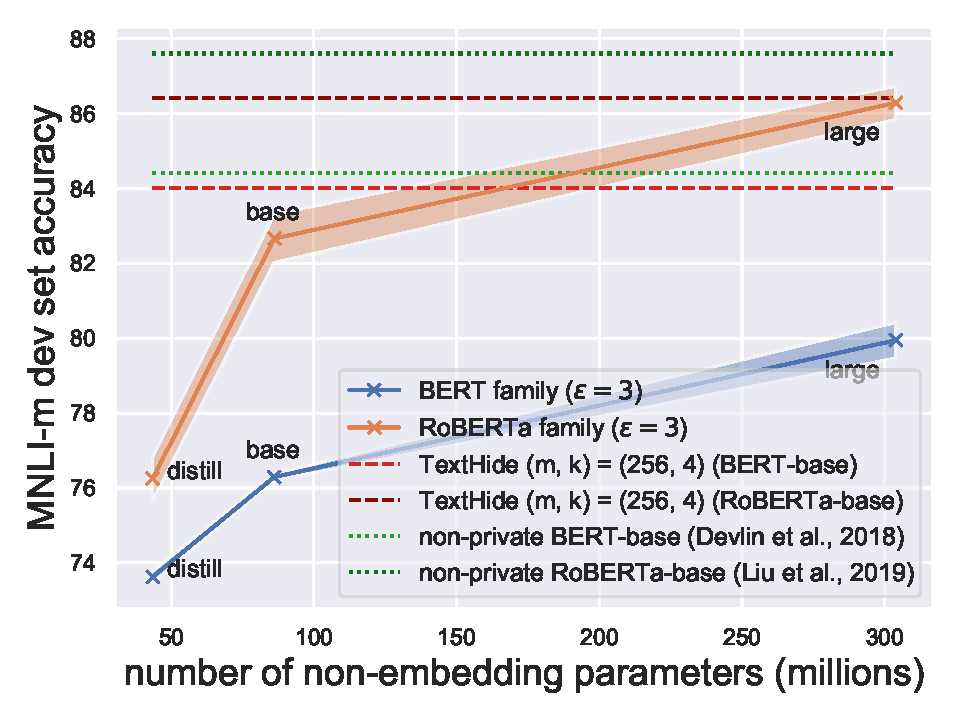
\includegraphics[width=0.98\textwidth]{figs/figure1_classification_v2.pdf}}
(a) Sentence classification \\MNLI-matched~\citep{williams2018multi}
\end{minipage}
\begin{minipage}[t]{0.48\linewidth}
\centering
{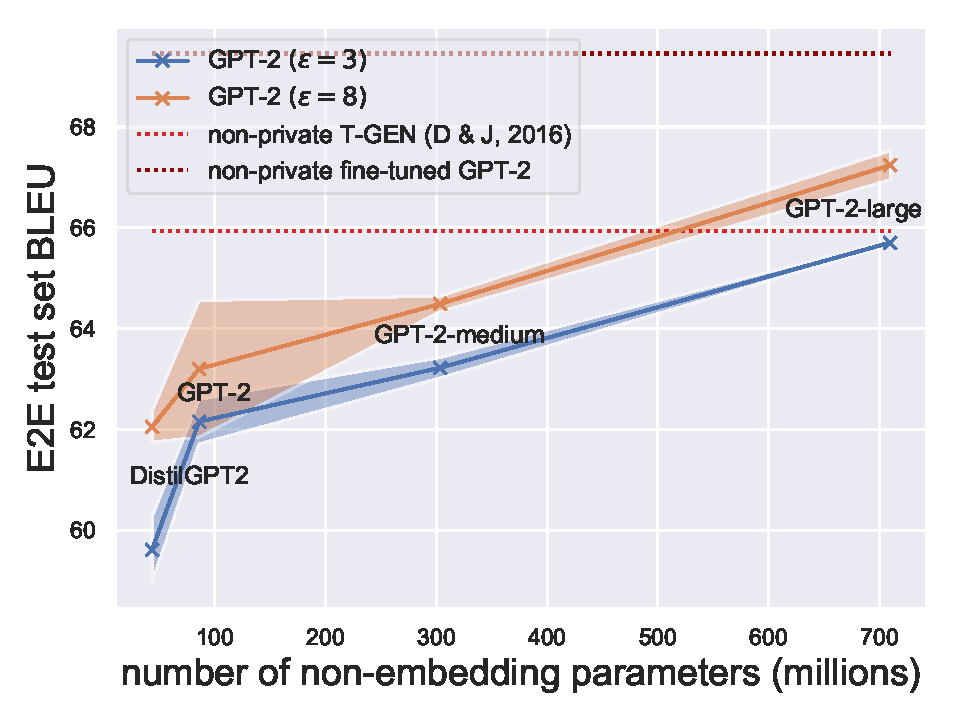
\includegraphics[width=0.98\textwidth]{figs/figure1_generation.pdf}}
(b) Natural language generation \\E2E~\citep{novikova2017e2e}
\end{minipage}
\end{center}
\caption{A summary of a few of our findings:
(1) Pretrained models fine-tuned with DP-Adam has strong performance. 
(2) Fine-tuning larger models produces better results. 
(3) Fine-tuned RoBERTa-large under DP at $\epsilon=3$ outperforms TextHide (the extension of InstaHide~\citep{huang2020instahide} for text classification) with BERT-base. 
Non-private generation baseline numbers are based on those reported by~\cite{wiseman2018learning}. 
}
\label{fig:fig1}
\end{figure}

\section{Problem Statement}
We build models for sentence classification and language generation tasks with datasets of modest sizes under (central/global) $(\epsilon, \delta)$-DP~\citep{dwork2014algorithmic}.

Intuitively, DP algorithms ensure that random outputs obtained from similar inputs are difficult to distinguish. 
$\epsilon$ and $\delta$ are \textit{privacy leakage} parameters that measure the loss of privacy and small values imply stronger privacy guarantees.
Unlike heuristic privacy notions~\citep{huang2020instahide}, DP allows for the tracking of privacy loss through the calculation of leakage parameters, and ensures privacy under composition~\citep{dwork2014algorithmic}, meaning that the overall privacy loss of multiple DP algorithms releasing multiple statistics can be reasoned in a principled manner.

DP learning typically relies on DP optimizers which privatize gradients before performing updates. 
The privatization step ensures that parameter updates leak limited information about training examples through their gradients.
Specifically, this step clips per-example gradients with a norm constraint $C$, and adds Gaussian noise $z\sim\mathcal{N}(0, C^2\sigma^2 I_p)$ to the sum of clipped gradients.
Here, $\sigma$ is the \textit{noise multiplier} determined from the privacy budget $(\epsilon, \delta)$, number of gradient updates $S$, and sampling rate $q=\tfrac{B}{N}$ for a batch size of $B$ and a dataset size of $N$.\footnote{Since we adopted the definition of ``neighboring'' based on addition/removal, the batch size here should be interpreted as the lot size~\citep{abadi2016deep} or, equivalently stated, the expected size of a batch drawn with Poisson sampling.}
Intuitively, clipping individual gradients ensures that each example has bounded influence on the parameter update, whereas noising the gradient prevents exact tracing of particular examples.
The noise being isotropic implies that larger models would experience heavier noise per update, as the norm of the $p$-dimensional Gaussian $\normtwo{z}$ scales as $C \sigma \sqrt{p}$.
This is widely believed to be the cause for DP optimization to perform poorly at training high-dimensional deep learning models~\citep{gautum14,yu2021not}.

Our starting point for building DP language models is (public) pretrained models. 
Pretrained language models tend to contain general knowledge of language~\citep{manning2020emergent} and thus should make the downstream private learning problem easier.
We fine-tune these models with DP-Adam~\citep{abadi2016deep,kingma2014adam} (see Chapter~\ref{sec:dp_first_order} for details) and track privacy loss through R\'enyi DP~\citep{mironov2017renyi}, but also report the converted $\epsilon$ from a Gaussian DP central limit theorem~\citep{dong2019gaussian} and from accurately composing tradeoff functions via fast Fourier transform~\citep{gopi2021numerical}.
We consider privacy levels $\epsilon \in \{3,8\}$ and $\delta = \tfrac{1}{2 |\mathcal{D}_\text{train}|}$ throughout
for a training set of size $|\mathcal{D}_\text{train}|$.
We tune hyperparameters on a text generation task (E2E; introduced below) and transfer these to the remaining tasks.
We outline two broad classes of NLP problems considered in this paper and define what constitutes a record below.

\paragraph{Sentence classification.}
The goal is to learn a model that classifies sentences into one of a few categories.
For these tasks, each example/record consists of input sentences and a label to be predicted.
We fine-tune models of various sizes in the BERT~\citep{devlin2018bert} and RoBERTa~\citep{liu2019roberta} families, as these models are known to work well in non-private learning.

\paragraph{Language generation.}
The goal is to learn a model that generates natural language sentences given some context.
For table-to-text generation tasks such as E2E~\citep{novikova2017e2e} and DART~\citep{nan2020dart}, each example/record in the training data consists of a pair of table entry and corresponding text description to be predicted. 
For a dialogue generation task such as Persona-Chat~\citep{zhang2018personalizing}, each example/record consists of metadata, a dialogue history, and a response to be predicted. 
We fine-tune GPT-2~\citep{radford2019language} and variants of different sizes for these problems, as this model family is known to work well for text generation. 

\section{Effective Differentially Private Fine-Tuning}
By studying the impact of hyperparameters and choice of fine-tuning objective, we demonstrate that the performance of the DP-Adam baseline can be substantially improved, even matching some strong non-private learning results.
Our analyses reveal common failure modes when straightforwardly applying DP optimization and explain poor results reported in past works that consider these baselines.


\subsection{Hyperparameter Tuning}\label{sec:good_hyper_params}
DP optimization is sensitive to the choice of hyperparameters~\citep{papernot2019making}.
Our experiments suggest that its performance can vary from being close to that of random initialization with ill-chosen hyperparameters to near state-of-the-art with appropriately chosen ones. As a consequence, we present simple but effective guidelines on setting the most important hyperparameters.
Unless otherwise stated, the unmentioned hyperparameters are set to defaults documented in Appendix~\ref{app:good_hyper_params}. 

\subsubsection{Batch Size, Learning Rate \& Training Epochs}
Our experiments suggest that batch size is one of the most important hyperparameters to set correctly, and the dependence of the optimal batch size on the learning rate and training epochs makes its selection complex.
We first describe batch size selection in realistic, compute-bound settings and then describe how the complexity of identifying the optimal batch size in these situations arise due to constraints on the number of training epochs.

\begin{wrapfigure}[20]{r}{0.5\textwidth}
\centering
\vspace{-2mm}
{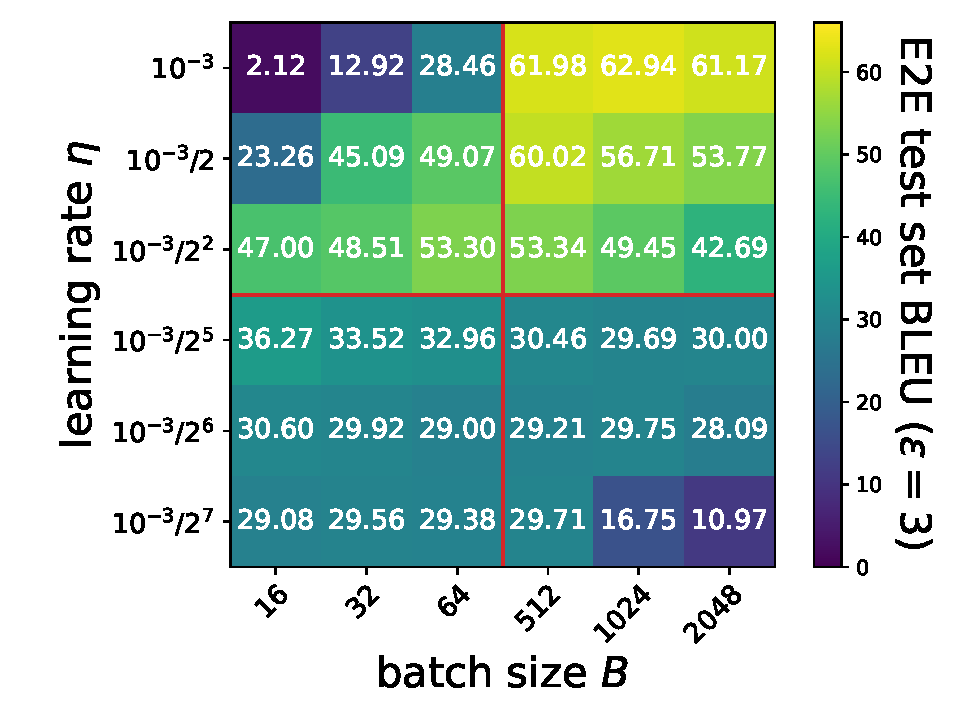
\includegraphics[width=0.45\textwidth]{figs/bs_vs_lr_BLEU.pdf}}
\caption{
Large batches and learning rates lead to good performance when the number of epochs is fixed.
Red lines divide heat map into four panels. Top and bottom correspond to low and high learning rate regimes; left and right correspond to small and large batch regimes.
Numbers are BLEU scores on the test split of E2E; higher is better.
}
\label{fig:bs_vs_lr}
\end{wrapfigure}
\paragraph{Fixed Training Epochs $E$.}
We first describe a very practical situation in which there is a constraint on the compute budget.
For the case of DP-SGD, this compute budget constraint often loosely translates to a constraint on the number of examples processed for gradient updates.\footnote{This is because DP-SGD often necessitates microbatching, in which case the number of backward passes is independent of the actual batch size for gradient updates but dependent on numbers of passes through the data.} 
In this fixed training epoch setting, the learning rate and batch size jointly affect performance, since using larger batches implies performing fewer gradient updates. 
To study this joint influence empirically, we fine-tune GPT-2 on the E2E dataset for table-to-text generation with DP-Adam at $\epsilon=3$ with various batch sizes and learning rates. 
Figure~\ref{fig:bs_vs_lr} shows that the best performing models (BLEU score \mytextapprox 62)
are obtained with both a large batch size and large learning rate. 
Using a small learning rate together with a small batch size yields considerably worse results. 
Note a seq2seq baseline achieves a test 
BLEU of \mytextapprox 65 without privacy here~\citep{wiseman2018learning}. 

Recall that in the non-private world, pretrained language models are typically fine-tuned with small batch sizes and small learning rates with Adam (bottom left panel in Figure~\ref{fig:bs_vs_lr}).
This implies that na\"ively fine-tuning pretrained language models privately using hyperparameters routinely used for non-private learning would degrade performance by more than necessary.\footnote{Anecdotally, moderately large learning rates also tend to work reasonably well in non-private learning. Small learning rates, however, are generally more stable, especially when (average) gradients aren't clipped.}

Recently, \cite{tramer2020differentially} studied how the batch size and learning rate jointly affect learning private image classifiers while holding other hyperparameters fixed.
They heuristically suggested a \textit{linear scaling rule}: Scaling the learning rate together with the batch size by the same constant should yield models with almost the same performance. 
However, Figure~\ref{fig:bs_vs_lr} indicates that this fails to hold consistently as it falsely predicts that large batch and high learning rate (top right entry) would have equal performance to small batch and low learning rate (bottom left entry).
We explain why linear scaling fails to predict performance for the small batch regime in Appendix~\ref{app:linear_scaling}. 

\paragraph{Fixed Update Steps $S$.}
In the fixed epoch setting, we saw that the optimal batch size was complex due to the trade-off between batch size and number of gradient updates.
We now show that the complexity of setting batch sizes arises almost entirely from this tradeoff by considering a different setting, where the total number of gradient updates (rather than epochs) is fixed.
In this case, using larger batches implies training for more epochs.

Here, we find that using larger batch sizes almost always results in better performance at a given privacy budget at the cost of processing more examples with more compute, once the other hyperparameters $S$, $\eta$, $C$, $\epsilon$, and $\delta$ are fixed.
We provide a heuristic explanation of this by introducing the idea of an \textit{effective noise multiplier} $\sigma_{\text{eff}} = \tfrac{\sigma}{q} = \tfrac{\sigma N} {B}$.  
Recall the noise multiplier $\sigma$ is determined from the privacy budget $(\epsilon, \delta)$, the number of update steps $S$, and the sampling rate $q$. 
In addition, recall the privatized gradient $\bar{g}$ in DP-SGD/DP-Adam which loosely takes the following form:
\eq{
\label{eq:sigma_eff_intuition}
	\bar{g} = \widetilde{g} + \widebar{z}
	, \quad
	\widetilde{g} = \frac{1}{B} \sum_{i \in \mathcal{B}} \text{Clip}(\nabla \mathcal{L}_i, C), \quad
	\widebar{z} \sim \mathcal{N} \Big(0, C^2 \tfrac{ \sigma^2}{B^2} I_p \Big) = \mathcal{N} \Big( 0, C^2 \tfrac{\sigma_{\text{eff}}^2}{N^2} I_p \Big),
}
where $\mathcal{B}$ is the Poisson-sampled batch of indices, $\nabla \mathcal{L}_i$ is the gradient of the $i$th example and $\text{Clip}(v, C) = v \cdot \min(1, \nicefrac{C}{\normtwo{v}} )$ clips the vector $v$ by the norm constraint $C$. 
We observe that for moderately large batches, the signal-to-noise ratio 
$r = \nicefrac{\normtwo{\widetilde{g}}}{\normtwo{\widebar{z}}}$ is mainly controlled by the batch size through the effective noise multiplier: 
The signal term $\widetilde{g}$ tends to concentrate quickly due to being an average of bounded vectors, whereas the effective noise multiplier $\sigma_{\text{eff}}$ decreases as the batch size $B$ increases (shown in Figure~\ref{fig:batch_size_fixed_t} (a)).
Figure~\ref{fig:batch_size_fixed_t} (b) plots the average signal-to-noise ratio $\widebar{r}$ over the first 30 gradient updates against the final model's performance on E2E and demonstrates that large batches (up to a threshold) correlates with both increased signal-to-noise ratio at the beginning of training and better performance at the end of training.
These findings additionally resonate with and explains recent empirical successes of large-scale private pretraining~\citep{anil2021large}.
\begin{figure}[htb]
\begin{center}
\begin{minipage}[t]{0.48\linewidth}
\centering
{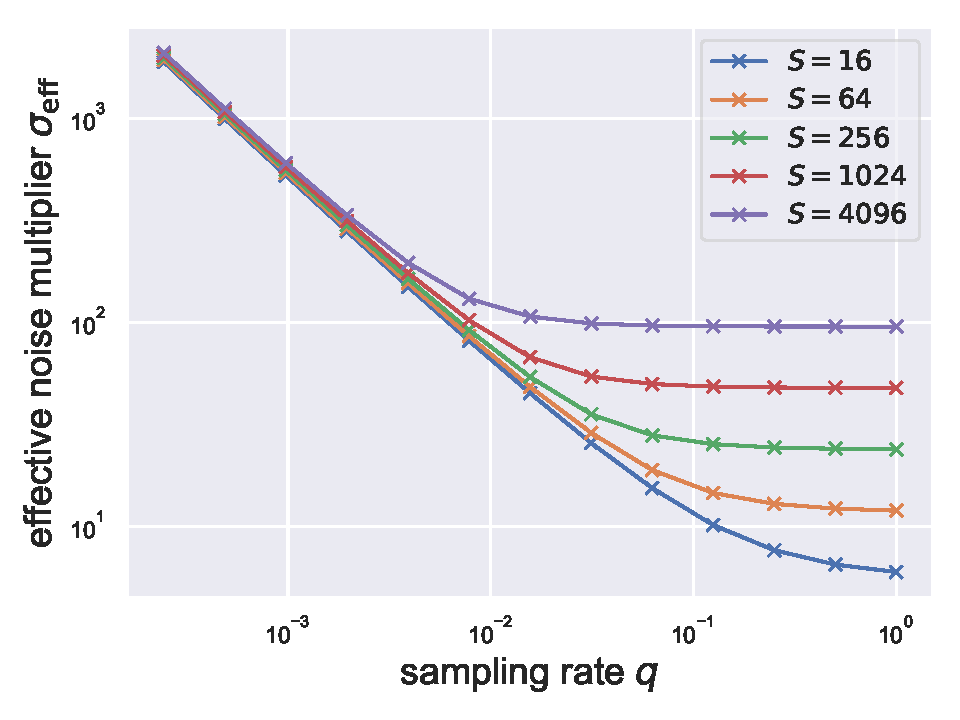
\includegraphics[width=0.98\textwidth]{figs/fixed_t_q_vs_sigma_eff_3.pdf}}
\end{minipage}
\begin{minipage}[t]{0.48\linewidth}
\centering
{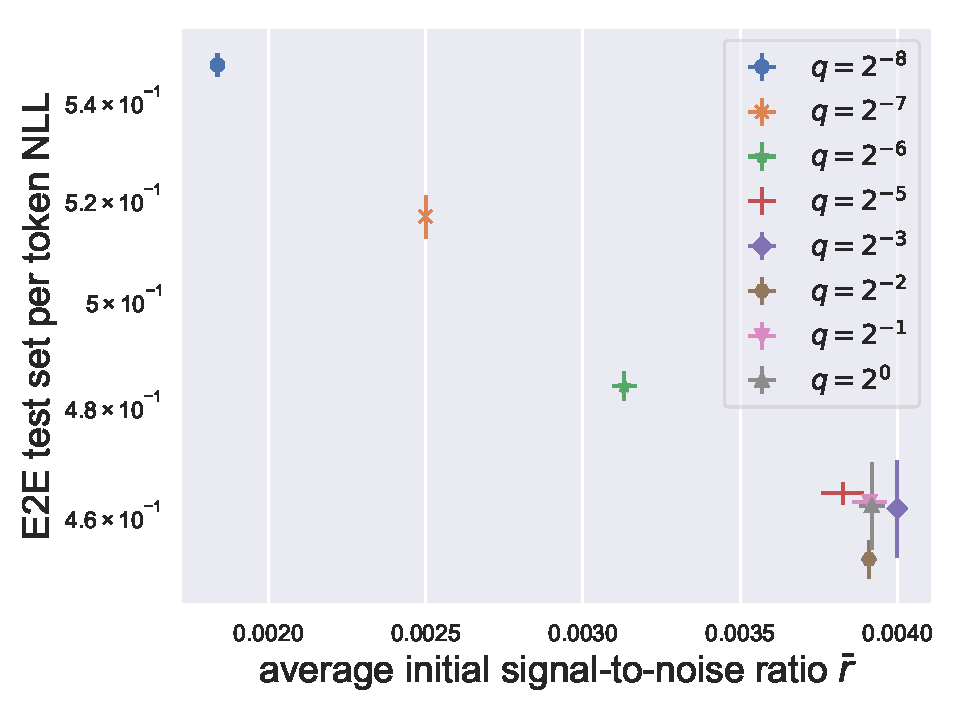
\includegraphics[width=0.98\textwidth]{figs/snr_vs_test_xent.pdf}}
\end{minipage}
\end{center}
\caption{
\textbf{Left:} Effective noise multiplier decreases with increasing sampling rate for various fixed number of updates $S$.
\textbf{Right:} Large batch sizes (corresponding to large $q$ in the figure) have higher signal-to-noise ratio at the beginning of training, which log-linearly correlates with final performance.
}
\label{fig:batch_size_fixed_t}
\end{figure}



\subsubsection{Clipping Norm}
DP optimization is known to be sensitive to the choice of clipping norm.
Since the scale of noise depends on this clipping norm (recall its standard deviation is $C \sigma$), picking the threshold $C$ much larger than the actual gradient norm implies more noise is being applied than necessary.
In practice, we have found that a small clipping norm which enforces almost all gradients to be clipped throughout training leads to the best performing models; see Figure~\ref{fig:app_hyperparameter}.

\begin{figure}[H]
\begin{center}
\begin{minipage}[t]{0.48\linewidth}
\centering
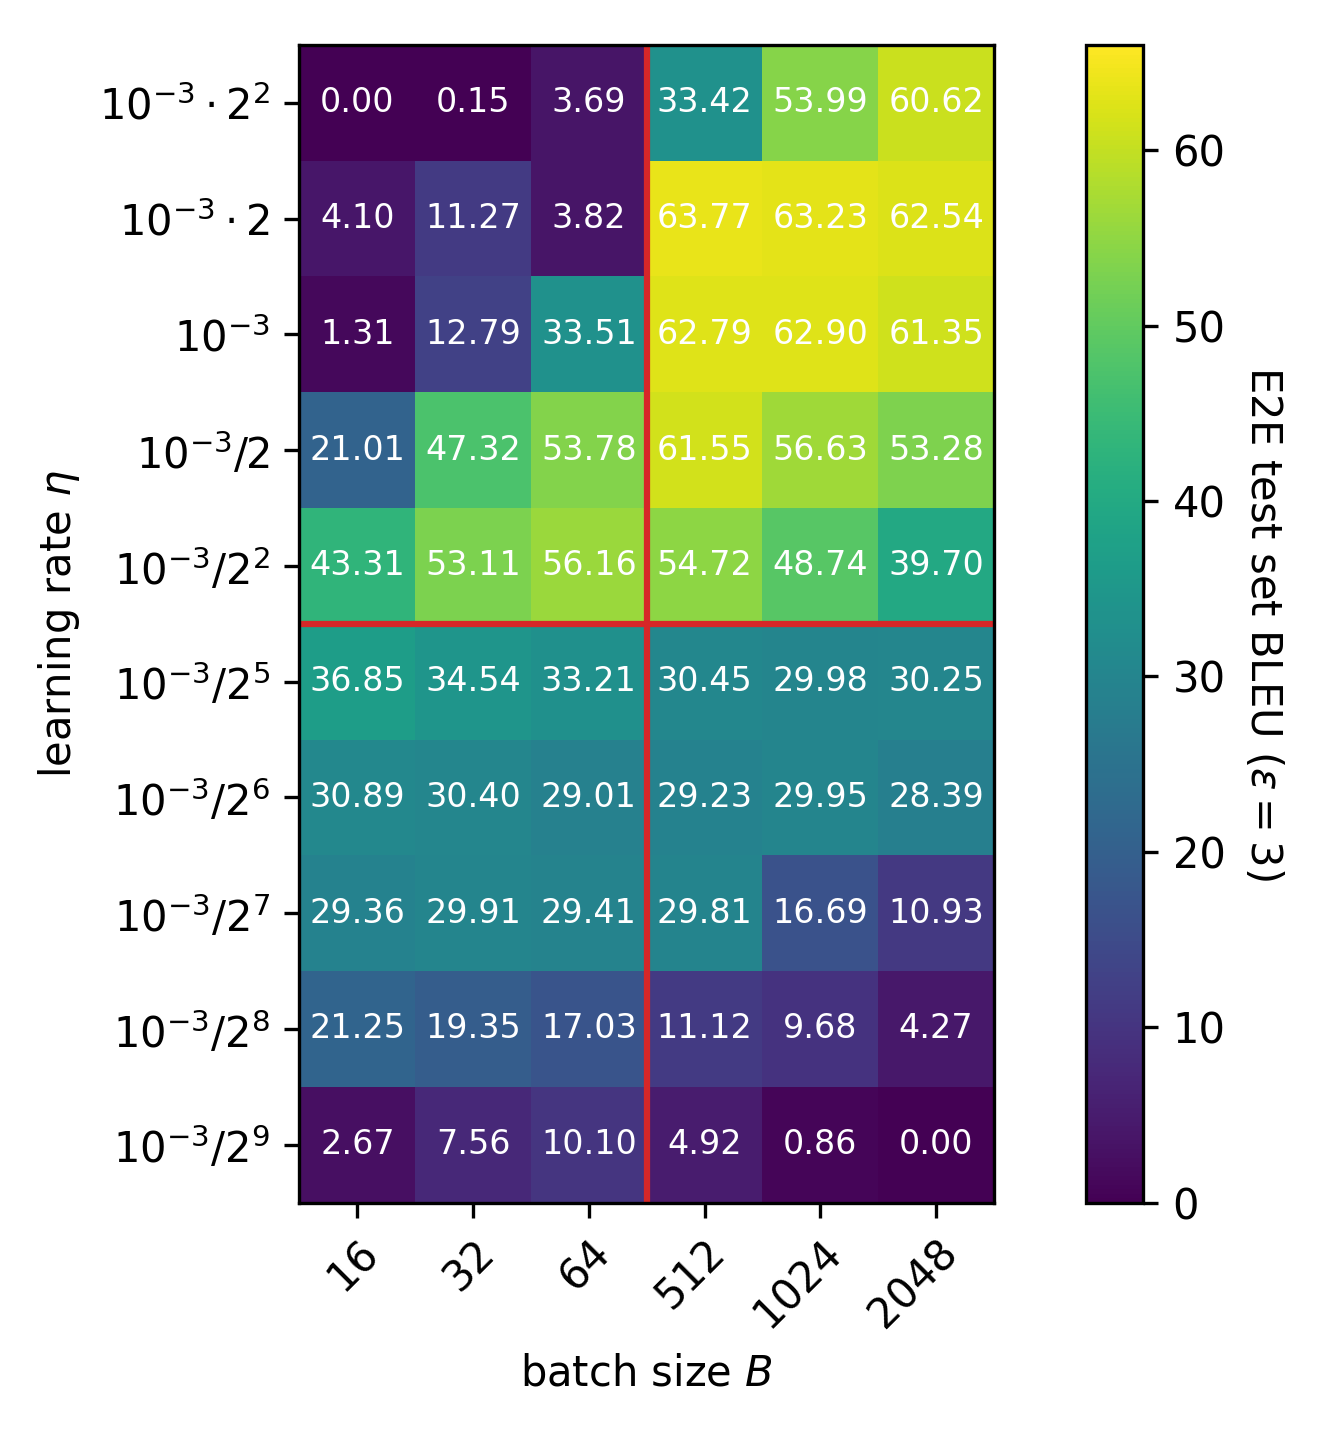
\includegraphics[width=0.96\textwidth]{figs/bs_vs_lr_BLEU_v2_cropped.png} \\ \vspace{-0.10cm}
(a) Batch size.
\end{minipage}
\begin{minipage}[t]{0.48\linewidth}
\centering
{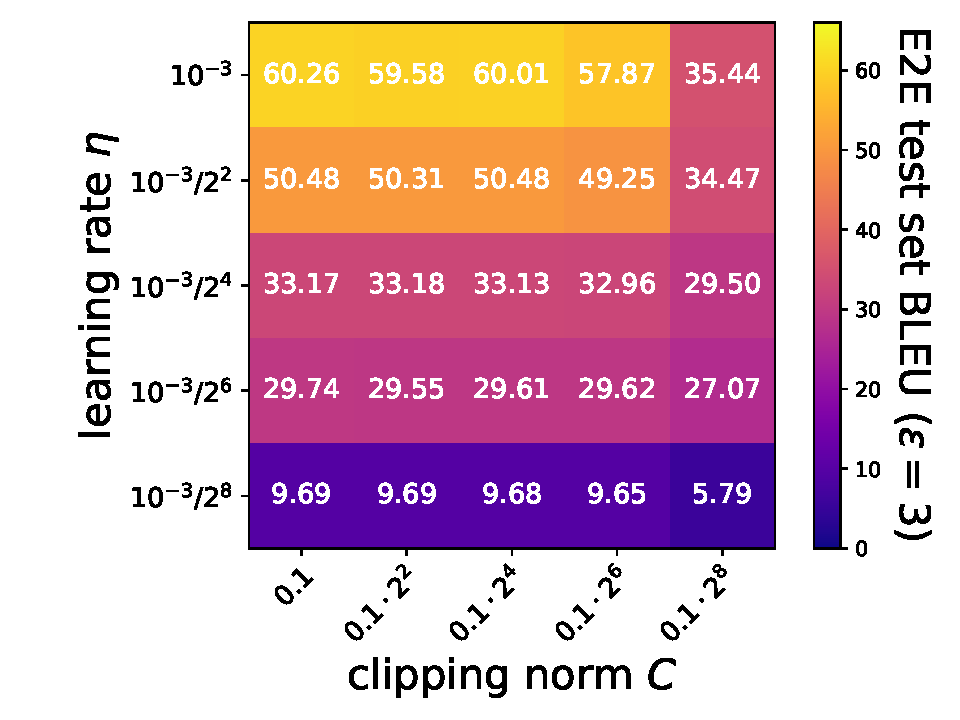
\includegraphics[width=0.96\textwidth]{figs/cn_vs_lr_BLEU.pdf}} \\ \vspace{-0.10cm}
(b) Clipping norm. 
\end{minipage}
\end{center}
\caption{Additional results on hyperparameter sensitivity.}
\label{fig:app_hyperparameter}
\end{figure}


\subsection{Improving the task alignment helps private learning}\label{sec:task_alignment}
Our fine-tuned models on language generation tasks work well since the pretraining objective and downstream task are \emph{aligned}: Both involve predicting sequences of tokens.
This alignment simplifies the task and benefits private learning. 
While pretrained models are naturally aligned for language generation, it is much less so for classification tasks. The standard approach for adapting language models for classification involves stacking a freshly initialized network on top of the encoding of the special \texttt{[CLS]} token and jointly optimizing all parameters~\citep{devlin2018bert}. 
This workflow introduces a discrepancy between pretraining and fine-tuning: Pretraining predicts masked out words from a large vocabulary whereas fine-tuning predicts integer labels.

To eliminate the discrepancy, we instead consider learning to predict the missing word during fine-tuning for classification. 
For example, for sentiment classification, we reframe the problem as filling in the \texttt{[MASK]} token in the sequence ``\texttt{<INPUT>}. It is \texttt{[MASK]}.'' and compare the probabilities of words ``awesome'' and ``terrible''.
This text infilling task is almost exactly the procedure used for pretraining masked language models, and recent works have demonstrated its effectiveness for knowledge probing~\citep{petroni2019language}, few-shot learning~\citep{gao2020making} and multi-task fine-tuning~\citep{wei2021finetuned}. 
On SST-2, we found that using the generic template as described above already improved private fine-tuning performance by $3\sim5\%$ across different settings.
Table~\ref{table:glue} (to be presented) contains additional results and Appendix~\ref{app:task_alignment} includes analyses on choices of label words.



\section{Ghost Clipping: Clipping without per-example gradients}
DP-SGD has high memory overhead due to clipping \textit{per-example} gradients.
Na\"ively implemented, this step instantiates a giant gradient vector for each example during optimization and can be prohibitively expensive.
For example, \cite{hoory2021learning} pretrained BERT with DP optimization and reported memory issues when using the large batches necessary to achieve high performance.
A time-costly solution to the memory problem is micro-batching: Split large batches into multiple smaller ones and aggregate the results after processing each small batch individually~\citep{tramer2020differentially}.
This solution, however, is unlikely to be sufficient as neural language models become larger and fitting even a few copies of the gradient in memory can be difficult.
\cite{lee2020scaling} observed that per-example gradients need not be instantiated at all, if the goal is to sum the clipped gradients. 
They presented a clipping procedure that only instantiates the per-example gradient for parameters of a \textit{single} layer in the model one at a time, as opposed to the entire model at once, at the cost of an extra backpropagation pass per processed batch. 


Unfortunately, we find this trick to be still insufficient for sequence models such as Transformers~\citep{vaswani2017attention}, as the memory requirement for per-example gradients of embedding layers and language modeling heads can be costly. We extend the \cite{lee2020scaling} approach such that training Transformers with DP optimization can have almost the same memory consumption as non-private training. 
Unlike their approach, our extension avoids instantiating the per-example gradient even for individual linear layers.
We call this approach \textit{ghost clipping}, as the per-example gradient is the ghost that never explicitly appears.
We anticipate this extension to be useful for both privately fine-tuning and pretraining large Transformers.

\subsection{The memory trick by~\cite{lee2020scaling}}
Per-example gradient clipping is easy if we know per-example gradient norms. In this case, we first compute the scaling factor $c_i = \min(1, \nicefrac{C}{ \normtwo{ \nabla \mathcal{L}_i} })$, where $C$ is the clipping threshold and $\mathcal{L}_i$ is the loss associated with the $i$th example. Then, we perform the usual backward pass with the reweighted scalar loss $ \sum_{i} c_i \mathcal{L}_i $. This procedure gives us the sum of clipped gradients.
Under this setup, the difficulty is computing the per-example gradient norm $\normtwo{\nabla \mathcal{L}_i}$. 
We emphasize two technicalities that enable computing this quantity without instantiating the full per-example gradient $\nabla \mathcal{L}_i$. 

First, for a typical neural net layer $l$ with parameters $W^{(l)}$ (without parameter sharing), the per-example gradient w.r.t. parameters can be easily computed using the input to the layer $a^{(l)}$ and the gradient of the loss w.r.t. the output $g^{(l)}$, both of which are available during backpropagation. 
Second, for a large vector formed by concatenating several small vectors $u = [u_1, \dots, u_k]$, its Euclidean norm is simply the norm of the vector of norms, i.e. 
$
\normtwo{ u } =
    \normtwo{ ( \normtwo{u_1}, \dots, \normtwo{u_k} ) }. 
$
The second observation means that computing the per-example gradient norm $\normtwo{\nabla  \mathcal{L}_i}$ can be done by computing the per-example gradient norms for individual layers of the neural net $\normtwo{\nabla_{W^{(1)}}  \mathcal{L}_i}, \dots, \normtwo{\nabla_{W^{(L)}}  \mathcal{L}_i}$ one at a time ($L$ is layer count). 
Moreover, the first observation implies that the norms for each layer can be computed using quantities freely available to a typical backward pass.
Overall, the per-example gradient norm of any network without parameter sharing can be computed in a layer-by-layer fashion with only one per-example gradient tensor for a single layer being instantiated at any time. 




\subsection{Ghost clipping for Transformers with sequential data}\label{sec:our_ghost}
The trick by~\cite{lee2020scaling} still requires instantiating the per-example gradient of individual layers (although not simultaneously). 
This can be problematic in terms of memory for Transformers with large embedding layers.\footnote{
	For GPT-2, per-example gradients w.r.t. the embedding for ten examples alone occupy \mytextapprox{1.5}GB of memory.
} 
Here, we present a specialized procedure for computing the per-example gradient norm for linear and embedding layers when they are applied to sequential data.\footnote{An embedding layer is essentially a linear layer: The embedding lookup operation applied to indices is equivalent to a matrix multiplication of the embedding matrix with one-hot encoded indices.}
This procedure reduces memory footprint and can be viewed as a generalization of the \cite{goodfellow2015efficient} trick that additionally handles sequential inputs. 

Let $a \in \R^{B\times T \times d}$ be the input to a linear layer with weight matrix $W \in \R^{p \times d}$, and $s \in \R^{B \times T \times p}$ be the output with $s_{i, j} = W a_{i, j}$. Let $g \in \R^{B \times T \times p}$ be the gradient of the loss w.r.t. the output $s$. 
Here, $T$ is the number of time steps in the input, and we omitted biases for simplicity. 
Simple calculation shows that the per-example gradient is the product of two matrices:
\eq{
\label{eq:seq_per_example_grad}
\nabla_{W} \mathcal{L}_i = g_i^\top a_i \in \R^{p \times d}. 
}
Since the per-example gradient norms are the end goal, the per-example gradients $\{\nabla_W \mathcal{L}_i\}_{i=1}^B$ themselves need not be instantiated explicitly. 
More precisely, we observe that the squared per-example gradient norm for this layer $\normf{\nabla_{W} \mathcal{L}_i}^2$ obeys the following key identity:
\eq{
\label{eq:better_per_example_grad}
\normf{ \nabla_{W} \mathcal{L}_i }^2 =
    \mathrm{vec}(a_{i} a_{i}^\top)^\top \mathrm{vec}( g_i g_i^\top ).
}
See Appendix~\ref{app:frobenius} for a derivation. 
Implemented with common primitives in machine learning libraries, \eqref{eq:better_per_example_grad} has a memory complexity of order $\mathcal{O}(BT^2)$ when $a_{i} a_{i}^\top\in\R^{T\times T}$ and $g_{i} g_{i}^\top\in\R^{T\times T}$ are instantiated,\footnote{The derived complexity is based on the assumption that the space complexity for multiplying two matrices $A\in \R^{m\times n}$ and $B\in \R^{n\times p}$ is roughly $\mathcal{O}(mp)$, which is the case for most workloads running on a framework like PyTorch. 
In addition, more sophisticated solutions may even avoid instantiating $a_{i} a_{i}^\top$ and $g_{i} g_{i}^\top$ entirely by trading in more run-time. Custom CUDA kernels are likely needed to make these solutions fast in practice.
} as opposed to $\mathcal{O}(Bpd)$ in the na\"ive approach which goes through instantiating \eqref{eq:seq_per_example_grad}.\footnote{We omitted the cost of storing $a_i$ and $g_i$, since our goal is to compare the additional cost induced by computing gradient norms.}

The memory efficiency of this procedure is exemplified with off-the-shelf pretrained language models, most of which have large embedding layers. 
For instance, for GPT-2, $d\approx50,000$ and $p=768$ for the embedding layer, and the context window $T\le 1024$.\footnote{In practice, for fine-tuning tasks, the maximum sequence length is usually a few hundred. } 
Our method in theory reduces the memory cost associated with this large embedding layer by at least a factor of $22$ compared to when the per-example gradient is na\"ively instantiated.
Overall, we also observe significant savings, since embedding layers can be a major source of memory spending for training large language models.\footnote{While there are alternative approaches for reducing the memory footprint of embedding layers during training,  
these methods tend to introduce extra hyperparameters that potentially require further tuning and privacy spending.
}

To stress-test ghost clipping, we compare it with $4$ baselines: The \texttt{PyTorch} package \texttt{Opacus} that implements DP optimization by instantiating per-example gradients, the approach by \cite{lee2020scaling}, non-private training in \texttt{PyTorch}, and na\"ive DP optimization implemented in \texttt{JAX} with \texttt{jit} and \texttt{vmap} enabled. 
We include the \texttt{JAX} baseline since a recent study showed that DP optimization can be made cheap through compiler optimization~\citep{subramani2020enabling}.
Figure~\ref{fig:ghost_clipping} (a) shows that for typical inputs, our technique is the most memory friendly and allows fitting batches almost as large as those in non-private training. 
Since ghost clipping allows us to fit larger batches but with a run-time penalty, a natural question is whether it improves throughput with the use of larger batches. 
Figure~\ref{fig:ghost_clipping} (b) shows that while ghost clipping only provides minor gains compared to \texttt{Opacus} for smaller models, it allows processing \mytextapprox{10\%} more examples compared to the approach by~\cite{lee2020scaling} for fitting GPT-2-large, a model that neither \texttt{Opacus} or \texttt{JAX} could handle. 
% See Appendix~\ref{app:memory} for the setup of these experiments.
\begin{figure}[htb]
\begin{center}
\begin{minipage}[t]{0.48\linewidth}
\centering
{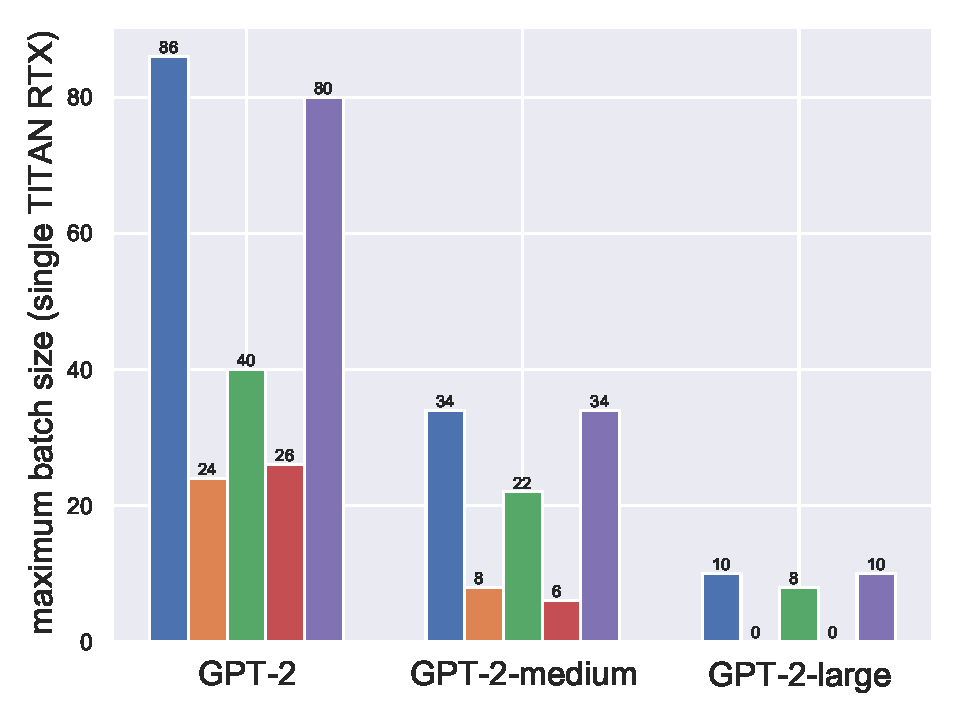
\includegraphics[width=0.98\textwidth]{figs/mem.pdf}}
(a) Memory
\end{minipage}
\begin{minipage}[t]{0.48\linewidth}
\centering
{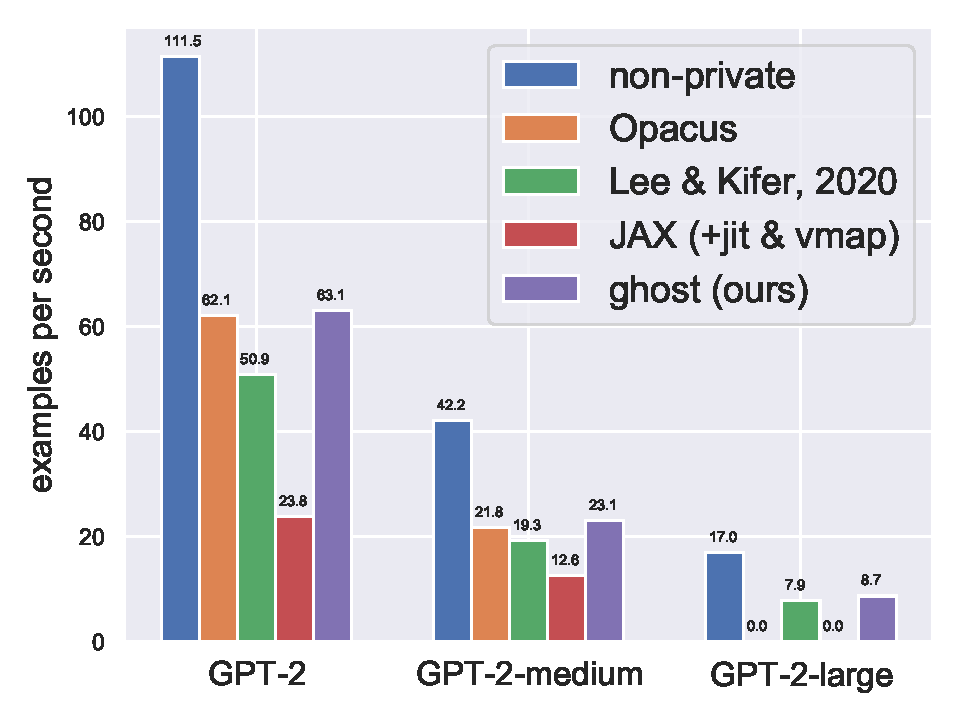
\includegraphics[width=0.98\textwidth]{figs/throughput.pdf}} 
(b) Throughput
\end{minipage}
\end{center}
\caption{
\textbf{Left:} 
Ghost clipping is 3 times more memory efficient than \texttt{Opacus} and is almost as efficient as non-private training for typical sequences across model sizes.
For GPT-2-large, we were unable to fit single-example micro batches together with gradient accumulation with \texttt{Opacus} or \texttt{JAX} on a TITAN RTX GPU ($24$ GBs of VRAM).
\textbf{Right:} DP optimization with ghost clipping processes \mytextapprox{10\%} more examples than the approach by~\cite{lee2020scaling} under unit time for GPT-2-large.
}
\label{fig:ghost_clipping}
\end{figure}

\section{Low Dimensionality Is Not Necessarily Better}\label{sec:dimensionality}
Since the norm of the noise injected into gradients during DP learning scales with dimensionality, it is natural to ask whether updating fewer parameters would result in improved performance.
We decompose this question into two aspects: (1) Do smaller pretrained models lead to better private fine-tuned performance, and (2) do parameter-efficient adaptation methods designed with a reduced dimensionality of updates outperform full fine-tuning?
Our experiments below show that neither is necessarily true.
Reported numbers in this section are averaged over three independent seeds.

\subsection{Larger Pretrained Models Result in Better Performance}
We observe that larger pretrained models lead to better private fine-tuned performance. 
Specifically, we fully fine-tune four sizes of GPT-2 models (for language generation) and three sizes of BERT/RoBERTa models (for sentence classification) at the same privacy budget with DP-Adam and compare their performances. 
Since the performance of DP optimization heavily depends on hyperparameter choices, we need to ensure that our hyperparameters are not particularly favoring larger models. 
We thus tune hyperparameters on the smallest model for each model type and then reuse the same hyperparameters for all fine-tuning workloads for that model type.
Figure~\ref{fig:fig1} from earlier demonstrates gains from model scaling on E2E and MNLI, and we find similar improvements on 5 additional tasks; see Figure~\ref{fig:fig1_extension}.

\begin{figure}[ht]
\begin{center}
\begin{minipage}[t]{0.45\linewidth}
\centering
{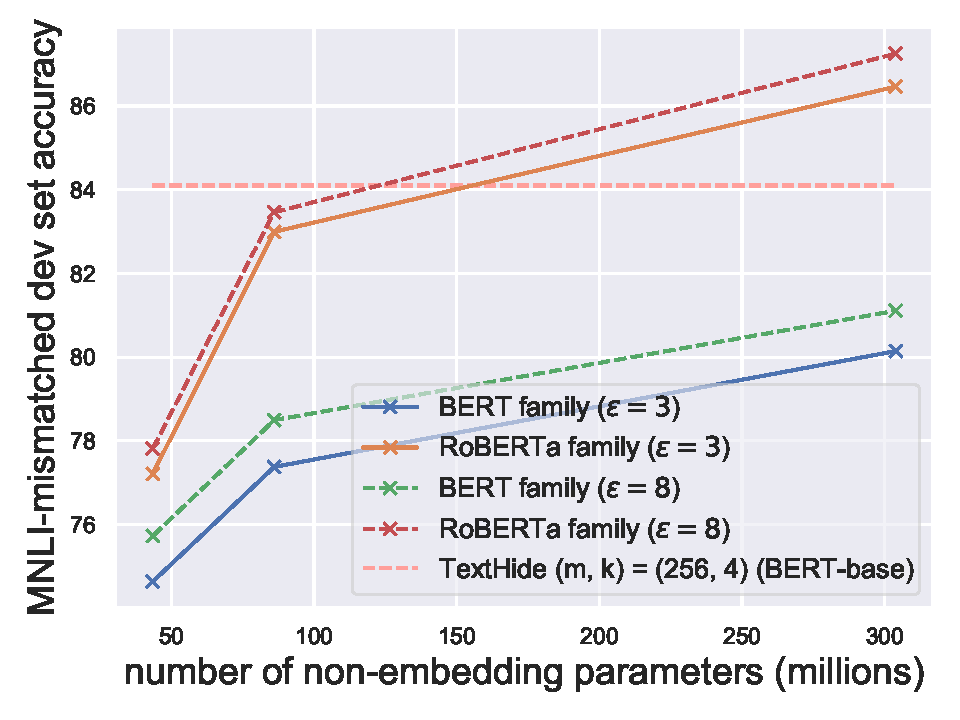
\includegraphics[width=0.98\textwidth]{figs/scaling-mnli.pdf}}
(a) MNLI-mismatched
\end{minipage}
\begin{minipage}[t]{0.45\linewidth}
\centering
{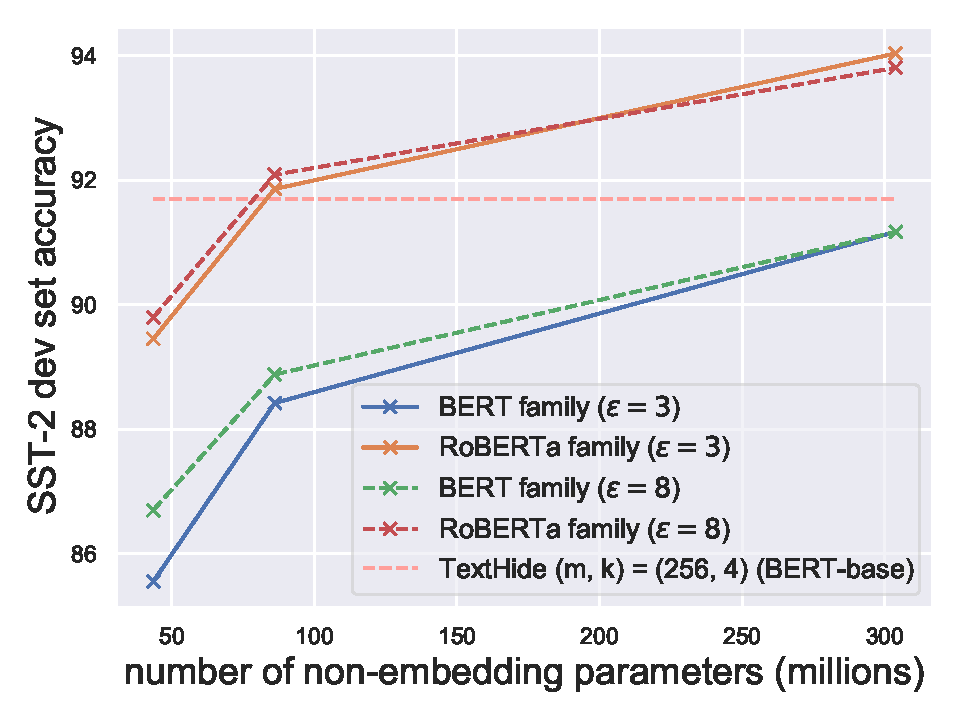
\includegraphics[width=0.98\textwidth]{figs/scaling-sst-2.pdf}}
(b) SST-2
\end{minipage}

\begin{minipage}[t]{0.45\linewidth}
\centering
{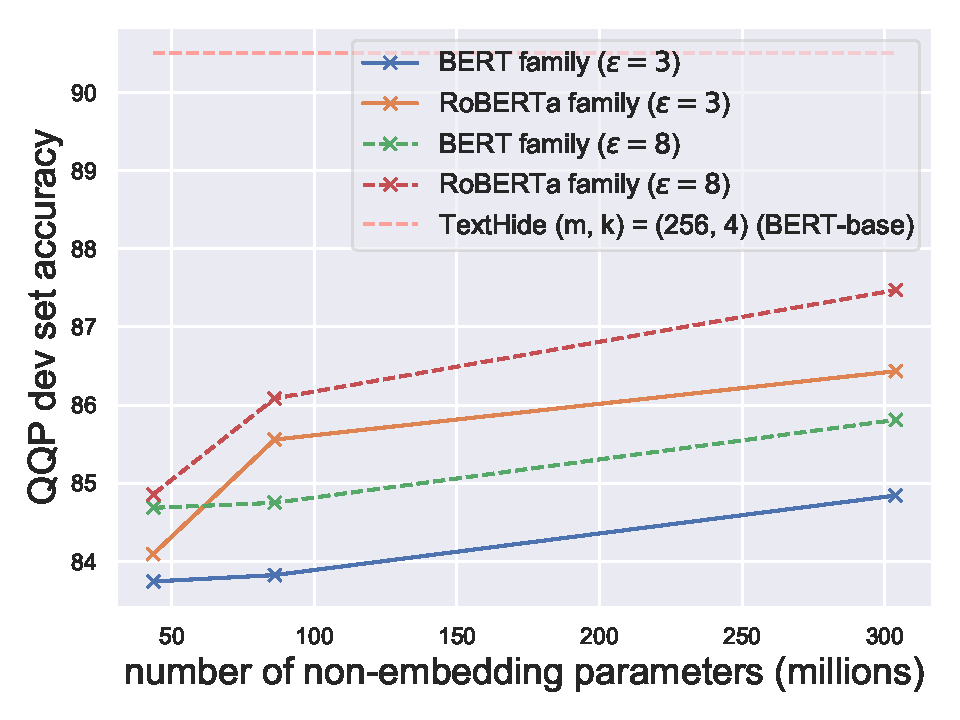
\includegraphics[width=0.98\textwidth]{figs/scaling-qqp.pdf}}
(c) QQP
\end{minipage}
\begin{minipage}[t]{0.45\linewidth}
\centering
{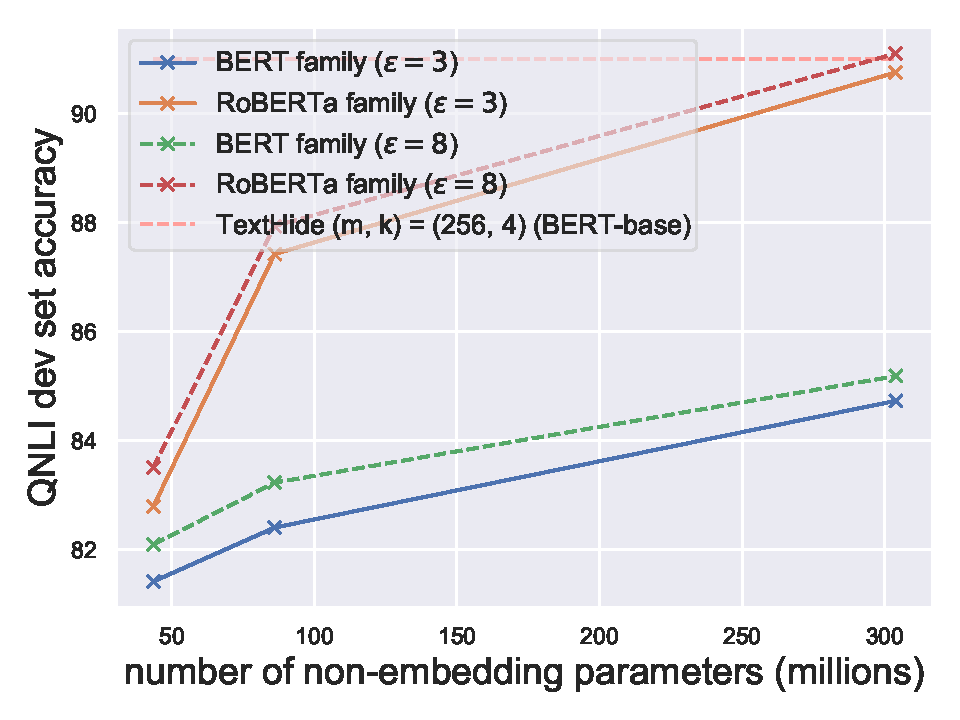
\includegraphics[width=0.98\textwidth]{figs/scaling-qnli.pdf}}
(d) QNLI
\end{minipage}
\end{center}

\begin{center}
\begin{minipage}[t]{0.45\linewidth}
\centering
{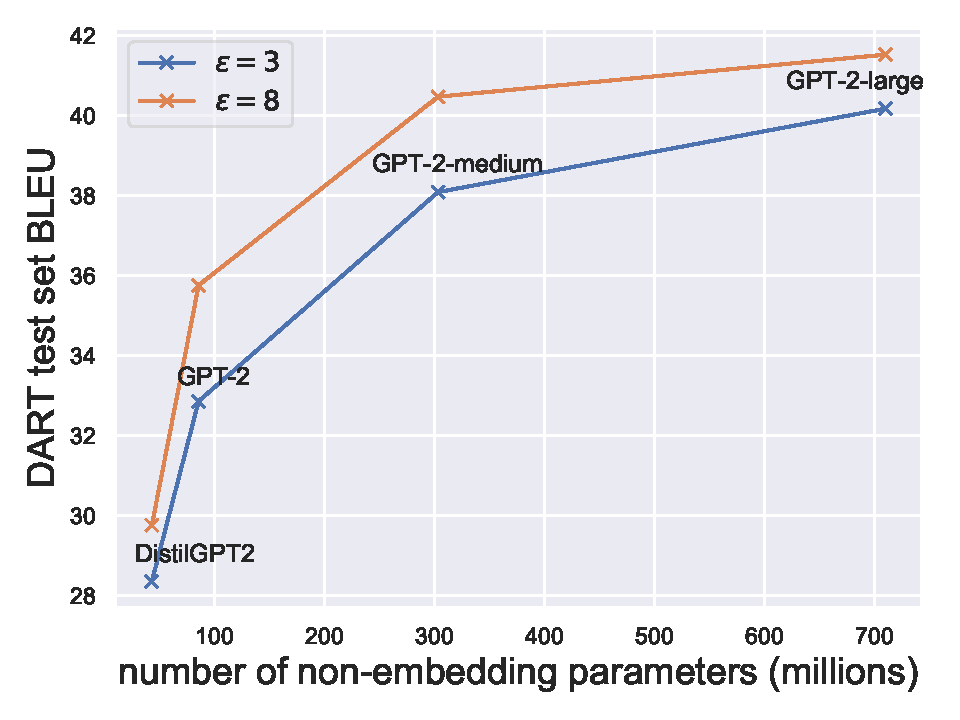
\includegraphics[width=0.98\textwidth]{figs/dart_scaling_BLEU.pdf}}
(e) DART
\end{minipage}
\end{center}

\caption{
Larger and better pretrained models consistently lead to better private fine-tuned performance on sentence classification and language generation tasks.
}
\label{fig:fig1_extension}
\end{figure}

\subsection[Full Fine-Tuning With DP-Adam Matches State-Of-The-Art]{\normalsize Full Fine-Tuning With DP-Adam Matches State-Of-The-Art}\label{sec:experiments_main}
There is a range of lightweight fine-tuning methods that reduce the dimensionality of updates, including some that are designed for DP~\citep{yu2021large}.
Do methods that optimize fewer parameters lead to better results under DP even if they perform similarly non-privately? Empirical results suggest otherwise and that full fine-tuning is a strong baseline that even matches specialized low-dimensional DP learning methods for both classification and generation.
Below, we study the two sets of tasks separately. 
For completeness, all experimental details are in Appendix~\ref{app:experiments_main}.

\paragraph{Sentence classification.}
We study DP fine-tuning on tasks from the GLUE benchmark that have more than $10$k training examples (MNLI, QQP, QNLI, and SST-2), following the experimental setup of~\cite{yu2021large}. 
The associated datasets have modest sizes: SST-2 and QNLI have 60k+ and 100k+ training examples, respectively. MNLI and QQP each contains less than 400k examples. 
Table~\ref{table:glue} shows that using larger pretrained models and the text-infilling objective generally improve classification accuracy. 
We compare full fine-tuning with \textit{reparameterized gradient perturbation} (RGP)~\citep{yu2021large}, as it is the state-of-the-art for DP fine-tuning on sentence classification at the time the first version of this paper was uploaded to arXiv. 
The method is designed to privatize gradients projected onto low dimensional subspaces and was motivated to reduce DP noise in high-dimensional models. 
We note that full fine-tuning with the text infilling objective outperforms well-tuned RGP on all tasks despite being the simplest baseline.\footnote{The careful reader will notice that the original RGP paper~\citep{yu2021large} reported considerably worse full fine-tuning results. We analyzed their released codebase and discovered a bug caused by their use of mixed-precision training. 
With this bug fixed, their codebase produces results similar to ours for full fine-tuning on SST-2. 
We detail subtleties of DP mixed-precision training in Appendix~\ref{app:mixed_precision}, and outline our implementation which achieves approximate scale invariance.
}
Computationally, while RGP is faster per-update, it requires more than 3 times as many epochs as full fine-tuning---overall, the two methods are comparable in terms of wall time. 
\begin{table}[th]
\footnotesize
\setlength\tabcolsep{2.4pt}
\caption{
Full fine-tuning larger pretrained models  with text infilling performs best.
Results are dev set accuracies. 
Bold numbers are the best for each privacy level based on two-sample test.
$\epsilon$ estimates based on numerically composing tradeoff functions.
}
\centering
\begin{tabular}{l cccc cccc}
\toprule
\multirow{2}[2]{*}{Method} 
& \multicolumn{4}{c}{\text{$\epsilon=3$}}
& \multicolumn{4}{c}{\text{$\epsilon=8$}} \\
\cmidrule(lr){2-5}
\cmidrule(lr){6-9}
 & MNLI-(m/mm) & QQP & QNLI & SST-2
 & MNLI-(m/mm) & QQP & QNLI & SST-2 \\
\midrule
RGP {(base)} & - & - & - & - & 80.5/79.6 & 85.5 & 87.2 & 91.6 \\
RGP {(large)} & - & - & - & - & 86.1/86.0	& 86.7 & 90.0 & 93.0 \\
\midrule
full (base)              & 82.47/82.10 & 85.41 & 84.62 & 86.12 & 83.30/83.13 & 86.15 & 84.81 & 85.89 \\
full (large)             & 85.53/85.81 & \textbf{86.65} & 88.94 & 90.71 & 86.28/86.54 & \textbf{87.49} & 89.42 & 90.94 \\
full + infilling (base)  & 82.45/82.99 & 85.56 & 87.42 & 91.86 & 83.20/83.46 & 86.08 & 87.94 & 92.09 \\
full + infilling (large) & \textbf{86.43/86.46} & 86.43 & \textbf{90.76}  & \textbf{93.04} & \textbf{87.02/87.26} & 87.47 & \textbf{91.10} & \textbf{93.81} \\
\midrule \midrule
$\epsilon$ &2.75 &2.75 &2.57 &2.41 &7.15 &7.16 &6.87 &6.69\\
\bottomrule
\end{tabular}
\label{table:glue}
\end{table}



\paragraph{Table-to-text generation.}
We study different fine-tuning methods under DP for table-to-text generation where the goal is to generate natural language descriptions of table entries. 
We consider the datasets E2E~\citep{novikova2017e2e} and DART~\citep{nan2020dart}. 
E2E consists of simple restaurant reviews, whereas DART consists of open-domain table entries from Wikipedia and is more complex. 
Both datasets are small: E2E has more than 40k training examples, whereas DART has more than 60k.
Since we are the first to experiment with this task under DP, we compare full fine-tuning (full) against a suite of parameter-efficient approaches which includes LoRA~\citep{hu2021lora}, prefix-tuning~\citep{li2021prefix} (prefix), RGP, and fine-tuning the top 2 Transformer blocks (top2), all of which optimize few parameters. 
On GPT-2 (125 million parameters), prefix-tuning with default hyperparameters optimizes \mytextapprox10 million parameters; LoRA with rank 4 optimizes \mytextapprox$0.15$  million parameters. 
We also report results for training from scratch (retrain).
Hyperparameters of each method were tuned only the E2E dataset; the complete search ranges are in Appendix~\ref{app:hp_search_range}.
Table~\ref{table:e2e_trim} shows that LoRA and full fine-tuning are generally the most performant on E2E. 
% Tables~\ref{table:e2e} and \ref{table:dart} in Appendix~\ref{app:table2text} contain the full result on E2E and DART and confirm the trend.
\setlength{\tabcolsep}{2.5pt}
\renewcommand{\arraystretch}{0.75}
\begin{table}[thb]
\footnotesize
\caption{
Full fine-tuning performs on par with or outperforms others methods that execute gradient update in low dimensional spaces.
Results are on E2E from fine-tuning GPT-2.
}
\centering
\begin{tabular}{l c c c cccccc}
\toprule
\multirow{2}[0]{*}{Metric} & \multirow{2}[0]{*}{DP Guarantee} & Gaussian DP & Compose & \multicolumn{6}{c}{Method}  \\
 & & + CLT & tradeoff func. & {full} & {LoRA} & {prefix} & {RGP} & {top2} & {retrain} \\

\midrule
\multirow{3}[1]{*}{BLEU}
 & $\epsilon=3$ & $\epsilon \approx 2.68$ & $\epsilon \approx 2.75$ & \textbf{ 61.519 } & 58.153 & 47.772 & 58.482 & 25.920 & 15.457\\
 & $\epsilon=8$ & $\epsilon \approx 6.77$ & $\epsilon \approx 7.27$ & \textbf{63.189} & \textbf{ 63.389 } & 49.263 & 58.455 & 26.885 & 24.247\\
 & non-private & - & - & 69.463 & 69.682 & 68.845 & 68.328 & 65.752 & 65.731\\
\midrule
\multirow{3}[1]{*}{ROUGE-L}
 & $\epsilon=3$ & $\epsilon \approx 2.68$ & $\epsilon \approx 2.75$ & \textbf{65.670} & \textbf{ 65.773 } & 58.964 & 65.560 & 44.536 & 35.240\\
 & $\epsilon=8$ & $\epsilon \approx 6.77$ & $\epsilon \approx 7.27$ & \textbf{66.429} & \textbf{ 67.525 } & 60.730 & 65.030 & 46.421 & 39.951\\
 & non-private & - & - & 71.359 & 71.709 & 70.805 & 68.844 & 68.704 & 68.751\\
\bottomrule
\end{tabular}
\label{table:e2e_trim}
\end{table}


\paragraph{Chit-chat dialog generation.}
We stress-test full fine-tuning under DP on the task of chit-chat dialog generation. This task has the distinct challenge that the response space is intrinsically diverse~\citep{li2015diversity,gao2018neural} since human conversations can be informal and noisy~\citep{zhang2019dialogpt}.
Moreover, dialog datasets are usually formed with user data which may contain sensitive information.
We use the Persona-Chat dataset \citep{zhang2018personalizing} as a testbed and build off a processed version that has \mytextapprox{130k} training entries.
Each entry contains a dialog history, persona descriptions of the respondent, and the response. 
We fine-tune GPT-2, GPT2-medium, and DialoGPT-medium on this dataset both privately and non-privately by training to predict the response with the dialog history and persona description. 
We report the F1 score and perplexity on the validation split, and human evaluated quality scores of generations.
Table~\ref{table:personachat} shows that private models have strong performance. 
In particular, fine-tuned DialoGPT-medium at $\epsilon=8$ beats the (non-private) winning entry of the ConvAI2 challenge~\citep{dinan2019second} on perplexity and has a human evaluation rating that is close to non-private models.
Samples from our private models can be found in Appendix~\ref{app:samples}.
\begin{table}[th]
\footnotesize
\setlength\tabcolsep{2pt}
\caption{
Fine-tuning with DP-Adam yields high quality chit-chat dialog generation models. 
}
\centering
\begin{tabular}{l c c c c c c}
\toprule
\multirow{2}[0]{*}{Model} & \multirow{2}[0]{*}{DP Guarantee} & Gaussian DP & Compose & \multicolumn{3}{c}{Metrics}  \\
 & & +CLT & tradeoff func. & \scriptsize{F1} $\uparrow$  & \scriptsize{Perplexity} $\downarrow$ & \scriptsize{Quality (human)} $\uparrow$ \\
\midrule
\multirow{3}[1]{*}{GPT-2}
& $\epsilon=3$ & $\epsilon \approx 2.54$ & $\epsilon \approx 2.73$ & 15.90 & 24.59  & - \\
& $\epsilon=8$ & $\epsilon \approx 6.00$ & $\epsilon \approx 7.13$ & 16.08 & 23.57  & - \\
& non-private  & - & - & 17.96 & 18.52  & - \\
\midrule
\multirow{3}[1]{*}{GPT-2-medium}
& $\epsilon=3$ & $\epsilon \approx 2.54$ & $\epsilon \approx 2.73$ & 15.99 & 20.68  & - \\
& $\epsilon=8$ & $\epsilon \approx 6.00$ & $\epsilon \approx 7.13$ & 16.53 & 19.25  & - \\
& non-private &- &- & 18.64 & 15.40  & - \\
\midrule
\multirow{3}[1]{*}{DialoGPT-medium}
& $\epsilon=3$ & $\epsilon\approx 2.54$ & $\epsilon \approx 2.73$ & \textbf{17.37} & \textbf{17.64}  & 2.82 (2.56, 3.09)\\
& $\epsilon=8$ & $\epsilon\approx 6.00$ & $\epsilon \approx 7.13$ & \textbf{17.56} & \textbf{16.79}  & 3.09 (2.83, 3.35)\\
& non-private &- &- & 19.28 & 14.28  & 3.26 (3.00, 3.51)\\
\midrule
HuggingFace {\scriptsize (ConvAI2 winner)} & non-private &-	&- & 19.09 & 17.51 & - \\
HuggingFace {\scriptsize (our implementation)} & non-private &- &- & 16.36 & 20.55 & 3.23 (2.98, 3.49) \\
\midrule
Reference &- &- &- &- &- & 3.74 (3.49, 4.00) \\
\bottomrule
\end{tabular}
\label{table:personachat}
\end{table}



\section{Related Work}

\paragraph{Private NLP.}
The privacy-preserving NLP space is largely divided by whether or not DP (or its extensions) is considered.
\cite{mcmahan2017learning} successfully trained small word-level RNNs with 1.35 million parameters in a federated setting with more than 700k users under a global DP guarantee with $(\epsilon, \delta) = (4.6, 10^{-9})$.
\cite{ramaswamy2020training} train production grade next-word prediction models using DP-FedAvg with millions of users.
\cite{qu2021privacy} studied fine-tuning BERT for language understanding tasks under local DP. 
\cite{kerrigan2020differentially} presented initial results that public pretraining is helpful for downstream DP fine-tuning.
However, they did not attempt fine-tuning large pretrained models with DP-SGD.
\cite{bommasani2021opportunities} briefly commented on the possibility of achieving cheaper private learning by fine-tuning large pretrained language models. 
\cite{anil2021large} pretrained BERT under global DP on datasets with hundreds of millions of examples. 
\cite{dupuy2021efficient} studied private BERT fine-tuning on datasets of utterances, but reported results with $\epsilon$ on the order of at least 100. 
Orthogonally, many works considered training language models that satisfy empirical notions of privacy~\citep{xu2021utilitarian,coavoux2018privacy,mireshghallah2021privacy,melamud2019towards}.
Our work is distinct from all works mentioned above in that we study fine-tuning large language models (with hundreds of millions of parameters) under global DP with stringent guarantees ($\epsilon \in \{3, 8\}$) on smaller datasets (much less than a million examples).

\paragraph{Differentially Private Deep Learning.}
DP-SGD has been viewed as ineffective for large models due to the addition of large Gaussian noise to gradient updates. 
Improvements to the learning procedure mostly fall under two distinct camps: $(i)$ Simplifying the private learning problem, and $(ii)$ reducing the scale of noise. 
For instance, \cite{papernot2019making,tramer2020differentially,abadi2016deep} consider transferring features learned on public datasets to simplify the subsequent private learning task. 
On the other hand, \cite{zhou2020bypassing,kairouz2020fast} remove the ambient dimension dependence of DP noise by identifying subspaces in which private gradients lie and would be privatized. 
\cite{yu2021not,yu2021large} make such ideas practical and demonstrate improved results on private learning benchmarks. 
\cite{zhang2021wide} applied the sparse vector technique to learning wide neural layers to reduce the amount of injected noise. 
Our work mostly falls under the first camp -- improving private learning through simplifying the learning task.
Our work is also distinct from prior works in that we focus on privately fine-tuning large pretrained models. 
Lastly, there are alternative solutions in the literature that enforces DP which are not based on gradient perturbation~\citep{papernot2018scalable,papernot2016semi}. 
These methods typically require extra public data and are not the present focus. 

\paragraph{Parameter-Efficient Fine-Tuning.}
Recent developments of pretrained model adaptation have produced a wide range of parameter-efficient fine-tuning methods for both vision and language tasks.
We briefly summarize these, grouping by category. 
Approaches based on optimizing prompt-like constructions for NLP tasks include prefix-tuning~\citep{li2021prefix}, P-tuning~\citep{liu2021gpt}, and prompt-tuning~\citep{lester2021power}.
Adapter-based methods insert small subnetworks inside pretrained Transformers~\citep{houlsby2019parameter,ruckle2020adapterdrop,pfeiffer2020adapterfusion}.
Methods that optimize low-rank matrices include the work by~\cite{hu2021lora,mahabadi2021compacter}.
In addition, there are adaptation methods that only optimize biases for vision~\citep{cai2020tinytl} and language tasks~\citep{ben2021bitfit}.
Our evaluation in Section~\ref{sec:experiments_main} covered the most representative methods that generally have state-of-the-art non-private learning performance (at the time of writing) for the range of NLP tasks studied in this paper.

\paragraph{Speeding Up DP-SGD.}
Apart from the work by~\cite{lee2020scaling} and~\cite{subramani2020enabling}, there is an approach that approximates per-example gradient norms through the combination of random projection and forward-mode autodiff~\citep{bu2021fast}.
While faster than vanilla private learning, this approach has the drawback of increased privacy spending and having an extra hyperparameter.
Our ghost clipping technique, while only suited for Transformers applied to sequential data, does not introduce new hyperparameters.

\paragraph{Alternative Clipping Strategies.}
While there are alternative clipping strategies in the literature that show improvements on simple tasks~\citep{pichapati2019adaclip,asi2021private}, we have opted to study the simplest strategy that clips gradients by their Euclidean norm.
We leave the study of these algorithms for NLP tasks to future work.

\paragraph{DP Synthetic Data Generation.}
Fine-tuning generative language models on private data under DP can also be viewed as a means of accomplishing DP synthetic data generation -- learning generative models from private data so that synthetic examples could be sampled and used for analysis. 
Previous work employed generative adversarial networks and focused primarily on image or tabular datasets~\citep{torkzadehmahani2019dp,neunhoeffer2020private,chen2020gs,torfi2020differentially}. 
Perhaps more related is the work by~\cite{bommasani19towards} which attempted fine-tuning GPT-2 on medical datasets to generate synthetic records but did not report any quantitative results. 


\section{Scope and Limitations}

We presented strategies for fine-tuning large pretrained language models under DP for a wide range of NLP tasks. 
For researchers and practitioners working on private NLP, our empirical results suggest that DP fine-tuning with a proper setup is a competitive baseline that is worth trying before prematurely shifting to less formal notions of privacy which have not stood against the test of time.
In addition, since DP fine-tuning generally requires substantially less private data (than training with DP from scratch), we hope this will motivate organizations which are already conducting private learning (e.g., federated learning with DP) to reduce the collection and use of private data to benefit privacy in the long run.
Below we list limitations and future directions. 

\paragraph{Public Pretraining.}
Our empirical studies are based on fine-tuning off-the-shelf models such as BERT and GPT-2 that are pretrained on data collected from the internet. 
Due to the permissive nature of the data collection for some of these models, there can be privacy concerns (e.g., text data scraped expansively from the internet may contain sensitive information such as PIIs~\citep{carlini2020extracting}).
We selected off-the-shelf models as they are widely accessible to ensure our results are reproducible.
When considering applying DP fine-tuning to real world settings, one should consider and create more curated public corpora for pretraining.

\paragraph{Hyperparameter Tuning.}
We studied how choices of basic hyperparameters affect the performance of DP-Adam for fine-tuning.
Our study is by no means comprehensive or complete.
In particular, we did not study how weight decay, learning rate schedule, clipping norm schedule, or batch size schedule affect private learning. 
Custom setups for these knobs have been found helpful for other private learning tasks~\citep{anil2021large}. 

Overall, our studies revealed that hyperparameter values can affect private fine-tuning in significant ways.
This calls for more transparency in reporting hyperparameter choices, analyses of hyperparameter transferability across tasks and architectures, and accounting of the privacy loss for hyperparameter tuning when hyperparameters aren't transferred across workloads.

\paragraph{Pretraining and Its Relation to Private Learning.}
Our model scaling results (Figure~\ref{fig:fig1}) suggest that using larger pretrained models improves performance. 
This argument, however, is dependent on the particular choice of pretrained models.
How pretraining helps private learning and whether better pretrained models for private learning could be built are interesting future avenues.

\paragraph{Scaling Laws for Private Learning.}
While scaling laws~\citep{kaplan2020scaling} for non-private deep learning have become prevalent, we are unaware of a case study in the private learning realm. 
Studies on how the dimensionality of models (and pretraining) generally affect private deep learning in precise terms will likely be a useful tool in trading off compute budget and model quality.


\chapter[Exploring the Limits of Differentially Private Deep Learning \\with Group-wise Clipping]{\Large Exploring the Limits of Differentially Private Deep Learning with Group-wise Clipping}\label{ch_4}
\chaptermark{Compute-Memory Tradeoff}

\chapter{When Does DP-SGD Not Suffer in High Dimensions?}

\chapter{Conclusion}\label{ch_6}

% long-term privacy leaks.
% language correlation, paper on not train privately on language
In this dissertation, we presented improved techniques for training deep learning models with DP that are more computationally efficient and have better privacy-utility trade-offs.
In addition, we also presented theoretical analyses that help explain and understand our seemingly counterintuitive empirical observations.
These contributions have gained industry adoption and have been deployed at Microsoft.
Below we discuss additional considerations.
\Chen{TODO: Logic of this chapter: 1) conclusions, 2) cautionary notes on DP limitation, 3) suggest that risk-benefit trade-off and long-term effect of deployment should be studied.}

\Chen{TODO: data collection harms.}

Successful private learning has the potential to motivate corporations to expand the deployment of DP machine learning.
This could result in long-term privacy harms that don't surface immediately.
For example, experiments in our work assume that the privacy budget $\epsilon$ is fixed ahead of time and model training is only ever performed once.
But for real-world deployments, statistical analyses or model training tend to be periodically repeated (with the same set of users) to adapt services to temporal changes in the data stream.
Some privacy is lost for each user with each repetition. \footnote{Foundation work has proposed the \emph{continual observation} model~\citep{dwork2010differential}; its deployment in privacy-preserving deep learning is yet to be seen.}

Lastly, we note that for DP algorithms to accomplish their privacy goal of ``hiding'' individuals' participation, one needs to assume that different examples in the dataset are produced independently~\citep{kifer2011no}.
When examples aren't independent, an algorithm can satisfy DP but still leak substantial privacy.\footnote{The simplest example is running DP algorithms on datasets with duplicates.}
Settings in our dissertation implicitly assumed that different examples are independent, but in practice example boundaries may be hard to define.
For instance, a transcript in a (private) dialog dataset can involve multiple users.
Defining the example boundary at the user level would imply that a transcript be duplicated across multiple users.
\Chen{TODO}
% Differential privacy as a guarantee alone may fail to fulfill the desired privacy goals if example boundaries are not set appropriately.

% We argue that improvements in differentially private machine learning alone should not be the sole motivation to
% expand the collection of user data or make aggressive the training of machine learning models on
% such data without considering the potential long-term harms of developing and releasing models
% trained with sensitive data.
% Our efforts on scaling differentially private fine-tuning to work with GPT-3 are purely motivated by
% an academic research question. We note there are privacy concerns associated with the pretraining
% corpus of GPT-3, and thus a model fine-tuned from GPT-3 should not be deployed without undergoing
% careful privacy audits. For deployment purposes, we suggest fine-tuning only models pretrained on
% carefully curated corpora.
% Lastly, we note that language is inherently complex, and its complexity may well be reflected in
% datasets for sophisticated tasks such as dialog completion. Differential privacy as a guarantee alone
% may fail to fulfill the desired privacy goals if example boundaries are not set appropriately.


% uncomment below if you have an appendix
% \appendix
% \chapter{A Long Proof}

\bibliographystyle{unsrt}  % can change to fit your field e.g. pnas2009
\bibliography{mybib}  % no .bib extension necessary

% adds a non-numbered signature page at end (for printing on ACID-FREE paper)
% (remember to comment out when submitting final version)
\onlinesignature

\end{document}
